% Options for packages loaded elsewhere
\PassOptionsToPackage{unicode}{hyperref}
\PassOptionsToPackage{hyphens}{url}
%
\documentclass[
]{book}
\usepackage{lmodern}
\usepackage{amssymb,amsmath}
\usepackage{ifxetex,ifluatex}
\ifnum 0\ifxetex 1\fi\ifluatex 1\fi=0 % if pdftex
  \usepackage[T1]{fontenc}
  \usepackage[utf8]{inputenc}
  \usepackage{textcomp} % provide euro and other symbols
\else % if luatex or xetex
  \usepackage{unicode-math}
  \defaultfontfeatures{Scale=MatchLowercase}
  \defaultfontfeatures[\rmfamily]{Ligatures=TeX,Scale=1}
\fi
% Use upquote if available, for straight quotes in verbatim environments
\IfFileExists{upquote.sty}{\usepackage{upquote}}{}
\IfFileExists{microtype.sty}{% use microtype if available
  \usepackage[]{microtype}
  \UseMicrotypeSet[protrusion]{basicmath} % disable protrusion for tt fonts
}{}
\makeatletter
\@ifundefined{KOMAClassName}{% if non-KOMA class
  \IfFileExists{parskip.sty}{%
    \usepackage{parskip}
  }{% else
    \setlength{\parindent}{0pt}
    \setlength{\parskip}{6pt plus 2pt minus 1pt}}
}{% if KOMA class
  \KOMAoptions{parskip=half}}
\makeatother
\usepackage{xcolor}
\IfFileExists{xurl.sty}{\usepackage{xurl}}{} % add URL line breaks if available
\IfFileExists{bookmark.sty}{\usepackage{bookmark}}{\usepackage{hyperref}}
\hypersetup{
  pdftitle={Fundamentos de Inferência Bayesiana},
  pdfauthor={Victor Fossaluza},
  hidelinks,
  pdfcreator={LaTeX via pandoc}}
\urlstyle{same} % disable monospaced font for URLs
\usepackage{longtable,booktabs}
% Correct order of tables after \paragraph or \subparagraph
\usepackage{etoolbox}
\makeatletter
\patchcmd\longtable{\par}{\if@noskipsec\mbox{}\fi\par}{}{}
\makeatother
% Allow footnotes in longtable head/foot
\IfFileExists{footnotehyper.sty}{\usepackage{footnotehyper}}{\usepackage{footnote}}
\makesavenoteenv{longtable}
\usepackage{graphicx,grffile}
\makeatletter
\def\maxwidth{\ifdim\Gin@nat@width>\linewidth\linewidth\else\Gin@nat@width\fi}
\def\maxheight{\ifdim\Gin@nat@height>\textheight\textheight\else\Gin@nat@height\fi}
\makeatother
% Scale images if necessary, so that they will not overflow the page
% margins by default, and it is still possible to overwrite the defaults
% using explicit options in \includegraphics[width, height, ...]{}
\setkeys{Gin}{width=\maxwidth,height=\maxheight,keepaspectratio}
% Set default figure placement to htbp
\makeatletter
\def\fps@figure{htbp}
\makeatother
\setlength{\emergencystretch}{3em} % prevent overfull lines
\providecommand{\tightlist}{%
  \setlength{\itemsep}{0pt}\setlength{\parskip}{0pt}}
\setcounter{secnumdepth}{5}
\usepackage{booktabs}
\usepackage[a4paper, top=3.5cm,bottom=2cm,inner=3.5cm,outer=2cm,headsep=1cm]{geometry}
\usepackage[brazil]{babel}
\usepackage[]{natbib}
\bibliographystyle{apalike}

\title{Fundamentos de Inferência Bayesiana}
\author{Victor Fossaluza}
\date{2020-08-11}

\begin{document}
\maketitle

{
\setcounter{tocdepth}{1}
\tableofcontents
}
Essas notas de aula tem o intuito apenas de ser um guia de estudos e não necessariamente irá apresentar todo o conteúdo da disciplina de \emph{Inferência Bayesiana}. Além disso, esta é uma versão preliminar e está bem longe de ser uma versão final, de modo que podem haver muitos erros e correções ou sugestões seráo bem vindas!

\hypertarget{ProbSubj}{%
\chapter{Probabilidade Subjetiva}\label{ProbSubj}}

A construção de probabilidade subjetiva apresentada aqui pode ser encontrada em \citet{DeGroot70}.

\begin{itemize}
\item
  \(\Omega\): \emph{espaço amostral}, conjunto não vazio.
\item
  \(\mathcal{A}\): \emph{\(\sigma\)-álgebra de subconjuntos} de \(\Omega\), isto é,

  \begin{enumerate}
  \def\labelenumi{\arabic{enumi}.}
  \tightlist
  \item
    \(\Theta \in \mathcal{A}\);
  \item
    \(A \in \mathcal{A} \Longrightarrow A^{c} \in \mathcal{A}\);
  \item
    \(\displaystyle A_1, A_2, \ldots \in \mathcal{A} \Longrightarrow \bigcup_{i\geq1} A_i \in \mathcal{A}\).
  \end{enumerate}
\item
  Os elementos de \(\mathcal{A}\) são chamados de \emph{eventos} e serão denotados por \(A, B, C, \ldots, A_1, A_2, \ldots\)
\end{itemize}

\hypertarget{definiuxe7uxe3o-axiomuxe1tica}{%
\section{Definição Axiomática}\label{definiuxe7uxe3o-axiomuxe1tica}}

\begin{itemize}
\tightlist
\item
  \(P: \mathcal{A} \longrightarrow [0,1]\) é uma \emph{medida de probabilidade} se

  \begin{enumerate}
  \def\labelenumi{\arabic{enumi}.}
  \tightlist
  \item
    \(P(\Omega) = 1\);
  \item
    \(\displaystyle A_1, A_2, \ldots \in \mathcal{A}\) com \(A_i \bigcap A_j = \emptyset\) , \(\displaystyle P\left(\bigcup_{i \geq 1} A_i\right) = \sum_{i \geq 1} P\left(A_i\right)\).
  \end{enumerate}
\end{itemize}

\hypertarget{interpretauxe7uxf5es-de-probabilidade}{%
\section{Interpretações de Probabilidade}\label{interpretauxe7uxf5es-de-probabilidade}}

\begin{itemize}
\tightlist
\item
  \textbf{Interpretação Clássica} (De Moivre, Laplace)

  \begin{itemize}
  \tightlist
  \item
    baseia-se na equiprobabilidade dos resultados;
  \item
    \(P(A) = \frac{|A|}{|\Omega|}\).
  \item
    \textbf{Exemplo:} um lançamento de moeda, \(A\) = ``cara'', \(P(A) = \frac{1}{2}\).
  \end{itemize}
\end{itemize}

\(~\)

\begin{itemize}
\tightlist
\item
  \textbf{Interpretação Frequentista} (Venn, von Mises, Reichenbach, etc.)

  \begin{itemize}
  \tightlist
  \item
    quase unânime na primeira metade do século XX e ainda é a mais aceita;
  \item
    baseia-se na regularidade das frequências relativas (lei dos grandes números);
  \item
    \(P(A) = lim \frac{A_n}{n}\), onde \(A_n\) é o número de ocorrências de \(A\) em \(n\) realizações \emph{idênticas e independentes} do experimento;
  \item
    Supõe que é possível repetir indefinidamente o experimento nas mesmas circustâncias.
  \item
    \textbf{Exemplo:} um lançamento de moeda, \(A\) = ``cara''.
  \end{itemize}
\end{itemize}

\begin{center}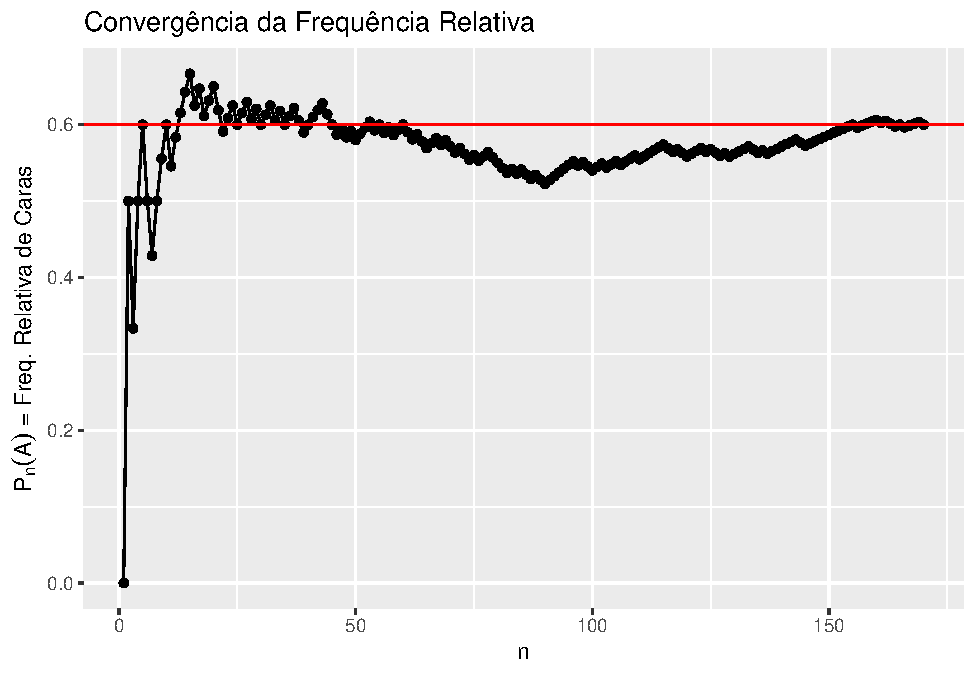
\includegraphics[width=0.7\linewidth]{InfBayes_files/figure-latex/unnamed-chunk-1-1} \end{center}

\(~\)

\begin{itemize}
\tightlist
\item
  \textbf{Interpretação Lógica} (Keynes, Jeffreys, Carnap, etc.)

  \begin{itemize}
  \tightlist
  \item
    medida de ``vínculo parcial'' entre uma evidência e uma hipótese;
  \item
    baseia-se em relações objetivas entre proposições.
  \item
    \textbf{Exemplo:} considere duas proposições: ``até agora todos os lançamentos resultaram em cara'' e ``será realizado um novo lançamento''. Pode-se afirmar que ``provavelmente o resultado do novo lançamento será cara''.
  \end{itemize}
\end{itemize}

\(~\)

\begin{itemize}
\tightlist
\item
  \textbf{Interpretação Subjetivista} (Ramsey, de Finetti, Savage, etc)

  \begin{itemize}
  \tightlist
  \item
    probabilidade como medida subjetiva de crença;
  \item
    baseada na experiência de cada indivíduo, portanto única.
  \item
    \textbf{Exemplo:} suponha que Bruno lançou uma moeda 3 vezes e todos os resultados foram cara. Esse indivíduo, em posse dessa informação, pode acreditar que o resultado cara é mais provável que coroa. Contudo, quando pergunta sobre a probabilidade de cara ao seu colega Olavo, ignorante com relação a moeda, ele responde que é 1/2.
  \end{itemize}
\end{itemize}

\(~\)

\hypertarget{relauxe7uxe3o-de-crenuxe7a-precsim}{%
\section{\texorpdfstring{Relação de Crença \(\precsim\)}{Relação de Crença \textbackslash precsim}}\label{relauxe7uxe3o-de-crenuxe7a-precsim}}

\(\precsim\) : relação de ``crença'' em \(\mathcal{A}\times\mathcal{A}\)

\begin{itemize}
\tightlist
\item
  \(A \prec B\) : acredito mais em \(B\) que em \(A\) (\(B \succ A\))
\item
  \(A \sim B\) : acredito igualmente em \(B\) e \(A\)
\item
  \(A \precsim B\) : acredito em \(B\) pelo menos tanto quanto em \(A\)
\end{itemize}

\textbf{Objetivo:} sob certas condições em \(\precsim\), obter uma medida de probabilidade \(P\) que representa (concorda) com \(\precsim\).

\[A \precsim B ~ \Longleftrightarrow ~ P(A) \leq P(B)\]

\hypertarget{suposiuxe7uxf5es-sobre-precsim}{%
\section{\texorpdfstring{Suposições sobre \(\precsim\)}{Suposições sobre \textbackslash precsim}}\label{suposiuxe7uxf5es-sobre-precsim}}

\textbf{SP1:} Para \(A, B \in \mathcal{A}\), exatamente uma das afirmações a seguir deve valer:\\
\[A \prec B ~,~ B \prec A ~\textrm{ou}~ A \sim B.\]

\(~\)

\textbf{SP2:} \(A_1, A_2, B_1, B_2 \in \mathcal{A}\) tais que \(A_1 \cap A_2 = B_1 \cap B_2 = \emptyset\) e \(A_i \precsim B_i\), \(i=1,2\). Então
\[A_1 \cup A_2 \precsim B_1 \cup B_2 .\]
Além disso, se \(A_i \prec B_i\) para algum \(i\), então \(A_1 \cup A_2 \prec B_1 \cup B_2 .\)

\(~\)

\textbf{SP3:} Se \(A\) é um evento, então \(\emptyset \precsim A\). Além disso, \(\emptyset \prec \Omega\).

\(~\)

\textbf{SP4:} Se \(A_1, A_2, \ldots\) uma sequência decrescente de eventos, isto é, \(A_n \supseteq A_{n+1}, \forall n\), e \(B\) tal que \(B \precsim A_n, \forall n\) então \[B \precsim \bigcap_{n \geq 1} A_n.\]

\(~\)

\textbf{SP5:} Existe uma variável aleatória \(X: \Omega \longrightarrow \mathbb{R}\), \(\mathcal{A}\)-mensurável, tal que \(X(\omega) \in [0,1], \forall \omega \in \Omega\) e, se \(I_1\) e \(I_2\) são intervalos contidos em \([0,1]\), \(\{X \in I_1\} \precsim \{X \in I_2\} \Leftrightarrow \lambda(I_1) \leq \lambda(I_2)~.\)

\begin{itemize}
\item
  Se \(I=[a,b] \subseteq [0,1]\), \(\lambda(I) = b-a\) é o comprimento do intervalo \(I\) (medida de Lebesgue).
\item
  ``Experimento auxiliar'' ; \(X \sim\) Uniforme{[}0,1{]}.
\item
  \(\{X \in [a,b]\}\) \(\sim \{X \in (a,b]\}\) \(\sim \{X \in [a,b)\}\) \(\sim \{X \in (a,b)\}\).
\end{itemize}

\(~\)

\textbf{Lema 1:} \(A, B, D \in \mathcal{A}\) tais que \(A \cap D = B \cap D = \emptyset\). Então \[A \precsim B ~\Leftrightarrow~ A \cup D \precsim B \cup D\]

\begin{quote}
\textbf{Demo:}\\
(\(\Rightarrow\)) \(A \precsim B \Rightarrow A \cup D \precsim B \cup D\) (SP2)\\
(\(\Leftarrow\)) \(B \prec A \Rightarrow B \cup D \prec A \cup D\) (SP2)
\end{quote}

\(~\)

\textbf{Teorema 1:} Se \(A \precsim B\) e \(B \precsim D\) então \(A \precsim D\).

\begin{quote}
\textbf{Demo:}
\end{quote}

\begin{center}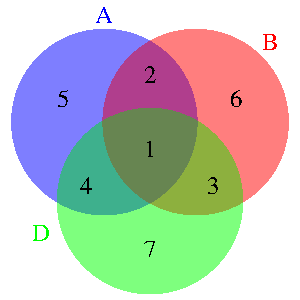
\includegraphics[width=0.7\linewidth]{InfBayes_files/figure-latex/Venn-1} \end{center}

\begin{enumerate}
\def\labelenumi{(\roman{enumi})}
\tightlist
\item
  \((1) \cup (2) \cup (4) \cup (5) \precsim (1) \cup (2) \cup (3) \cup (6)\) \(~\Rightarrow~ (4) \cup (5) \precsim (3) \cup (6)\).\\
\item
  Analogamente, \((2) \cup (6) \precsim (4) \cup (7)\)\\
  De (i) e (ii) e pelo Lema 1, \((4) \cup (5) \cup (2) \cup (6) \precsim (3) \cup (6) \cup (4) \cup (7)\)\\
  \(~\Rightarrow~ (2) \cup (5) \precsim (3) \cup (7)\) \({~\Rightarrow~ (2) \cup (5) \cup (1) \cup(4) \precsim (3) \cup (7) \cup (1) \cup(4)}\).
\end{enumerate}

\(~\)

\textbf{Teorema 2 (generalização do SP2):}
Se \(A_1, \ldots, A_n\) são eventos disjuntos e \(B_1, \ldots, B_n\) são também eventos disjuntos tais que \(A_i \precsim B_i\), para \(i=1,\ldots,n\), então \[\bigcup_{i=1}^{n} A_i \precsim \bigcup_{i=1}^{n} B_i.\]
Se \(A_i \prec B_i\) para algum i, então \(\bigcup_{i=1}^{n} A_i \prec \bigcup_{i=1}^{n} B_i.\)

\begin{quote}
\textbf{Demo:} Exercício.
\end{quote}

\(~\)

\textbf{Teorema 3:}
Se \(A \precsim B\) então \(A^c \succsim B^c\).

\begin{quote}
\textbf{Demo:} Do Lema 1, \(A \cup (A^c \cap B^c) \precsim B \cup (A^c \cap B^c)\) \(\Rightarrow B^c \cup (A \cap B) \precsim A^c \cup (A \cap B)\) \(\Rightarrow B^c \precsim A^c\).
\end{quote}

\(~\)

\textbf{Resultado:} Para todo evento \(A\), \(A \precsim \Omega\).

\begin{quote}
\textbf{Demo:} Por SP3, \(\emptyset \precsim A^c\). Tomando \(D=A\) no Lema 1, \(\emptyset \cup A \precsim A^c \cup A \Rightarrow A \precsim \Omega\).
\end{quote}

\(~\)

\textbf{Teorema 4:}
Se \(A \subseteq B\) então \(A \precsim B\).

\begin{quote}
\textbf{Demo:} Suponha, \(B \prec A\). Tomando \(D=B^c\) no Lema 1, \(B \cup B^c \prec A \cup B^c \Rightarrow \Omega \prec A \cup B^c\). Absurdo!
\end{quote}

\(~\)

\textbf{Exemplo 1:} \(\omega_0 \in \Omega\). \(A \precsim B \Leftrightarrow \{\omega_0 \in B\) \textbf{ou} \(\omega_0 \notin (A \cup B)\}\). Mostre que \(\precsim\) obedece a SP1 a SP4.

\begin{quote}
(SP1)\\
\(A \precsim B \Leftrightarrow \omega_0 \in B \cup (A \cup B)^c\)
\(\Rightarrow B \prec A \Leftrightarrow \omega_0 \in B^c \cap (A \cup B)\)
\(\Leftrightarrow \omega_0 \in A \cap B^c.\)\\
Analogamente, \(A \prec B \Leftrightarrow \omega_0 \in B \cap A^c.\)\\
\(A \sim B \Leftrightarrow A \precsim B\) e \(B \precsim A\)
\(\Leftrightarrow \omega_0 \in [B \cup (A \cup B)^c] \cap [A \cup (A \cup B)^c]\)
\(\Leftrightarrow \omega_0 \in (A \cap B) \cup (A \cup B)^c.\)\\
\(~\)\\
(SP2)\\
\(A_i \precsim B_i , i=1,2 \Leftrightarrow\) \(\omega_0 \in [B_1 \cup (A_1 \cup B_1)^c] \cap [B_2 \cup (A_2 \cup B_2)^c]\) \(\Leftrightarrow \omega_0 \in [(B_1 \cup B_2) \cap D^c] \cup (A_1 \cup B_1 \cup A_2 \cup B_2)^c,\)\\
com \(D = (A_1 \cap B2) \cup (A_2 \cap B1).\)\\
\(A_1 \cup A_2 \precsim B_1 \cup B_2 \Leftrightarrow\) \(\omega_0 \in (B_1 \cup B_2) \cup (A_1 \cup A_2 \cup B_1 \cup B_2)^c\)\\
Como \((B_1 \cup B_2) \cap D^c \subseteq (B_1 \cup B_2)\), vale o SP2.\\
\(~\)\\
(SP3)\\
\(\emptyset \precsim A \Leftrightarrow \omega_0 \in A \cup (\emptyset \cup A)^c\) \(\Leftrightarrow \omega_0 \in A \cup A^c = \Omega.\)\\
Como \(\Omega\) é não-vazio, \(\exists \omega_0 \in \Omega\) e, portanto, \(\emptyset \prec \Omega\).\\
\(~\)\\
(SP4) Exercício!
\end{quote}

\(~\)

\textbf{Exemplo 2:} \(\Omega = \mathbb{N}\), \(\mathcal{A} = \mathcal{P}(\mathbb{N})\). \(A \precsim B \Leftrightarrow \{B\) é infinito \textbf{ou} \(A\) e \(B\) são finitos com \(|A| \leq |B|\}\). Verifique se \(\precsim\) satisfaz SP1 a SP4.

\(~\)

\textbf{Teorema 5:} Se \(A_1 \subseteq A_2 \subseteq \ldots\) é uma sequência crescente de eventos e \(B\) é tal que \(A_n \precsim B, \forall n\) então \[\bigcup_{n \geq 1} A_n \precsim B.\]

\begin{quote}
\textbf{Demo:} \(A_n^c \supseteq A_{n+1}^c\) e, pelo Teo 3, \(A_n^c \succsim B^c\), \(\forall n\).\\
Por SP4, \(\bigcap_{n \geq 1} A_n^c \succsim B^c\) \(\Rightarrow \bigcup_{n \geq 1} A_n \precsim B.\)
\end{quote}

\(~\)

\textbf{Teorema 6:} \(\left(A_n\right)_{n \geq 1}\) e \(\left(B_n\right)_{n \geq 1}\) sequências tais que \(A_i \cap A_j = B_k \cap B_l = \emptyset\), \(\forall i \neq j\), \(\forall k \neq l\).
\[A_i \precsim B_i, \forall i ~\Rightarrow~ \bigcup_{n \geq 1} A_n \precsim \bigcup_{n \geq 1} B_n.\]
Se existe ao menos um \(j\) tal que \(A_j \prec B_j\) então \(\displaystyle{ \bigcup_{n \geq 1} A_n \prec \bigcup_{n \geq 1} B_n }.\)

\begin{quote}
\textbf{Demo:} Da extensão de SP2, temos que \(\displaystyle{ \bigcup_{i = 1}^n A_i \precsim \bigcup_{i = 1}^n B_i }\), \(\forall n \geq 1\) \(~\Rightarrow~ \displaystyle{ \bigcup_{i = 1}^n A_i \precsim \bigcup_{i = 1}^{\infty} B_i }\), \(\forall n \geq 1\) \(~\Rightarrow~ \displaystyle{ \bigcup_{i = 1}^{\infty} A_i \precsim \bigcup_{i = 1}^{\infty} B_i }~\) (Teo 5)\\
\(\exists n_0\) tal que \(A_{n_0} \prec B_{n_0}\). De SP2, temos que, para \(n \geq n_0\),\\
\(\displaystyle \bigcup_{i = 1}^{n_0} A_i = \bigcup_{i = 1}^{n_0-1} A_i \cup A_{n_0} \prec \bigcup_{i = 1}^{n_0-1} B_i \cup B_{n_0} = \bigcup_{i = 1}^{n_0} B_i\) \(~\Rightarrow~ \displaystyle \bigcup_{i = 1}^{n_0} A_i \prec \bigcup_{i = 1}^{n_0} B_i.\)\\
Da primeira parte, temos que \(\displaystyle{ \bigcup_{i = n_0+1}^{\infty} A_i \precsim \bigcup_{i = n_0+1}^{\infty} B_i } ~\) e, por SP2,\\
\(\displaystyle \bigcup_{i = 1}^{n_0} A_i \cup \bigcup_{i = n_0+1}^{\infty} A_i \prec \bigcup_{i = 1}^{n_0} B_i \cup \bigcup_{i = n_0+1}^{\infty} B_i\)\\
provando o resultado.
\end{quote}

\(~\)

\hypertarget{medida-de-probabilidade-que-representa-precsim}{%
\section{\texorpdfstring{Medida de Probabilidade que ``representa'' \(\precsim\)}{Medida de Probabilidade que ``representa'' \textbackslash precsim}}\label{medida-de-probabilidade-que-representa-precsim}}

\textbf{Teorema 7:} Seja \(A \in \mathcal{A}\). Então \(\exists! a^* \in [0,1]\) tal que \(A \sim \{X \in [0,a^*]\}\).

\begin{quote}
\textbf{Demo:} Seja \(U(A) = \left\{ a \in [0,1] : A \precsim \{X \in [0,a]\} \right\}\).\\
\(1 \in U(A)\) pois \(\Omega = \{X \in [0,1]\} \succsim A\) \(~\Rightarrow~ U(A) \neq \emptyset\).\\
Tome \(a^* = \inf U(A)\).\\
\(~\)\\
(i) Considere \((a_n)_{n \geq 1}\), \(a_n \in [0,1], \forall n \geq 1\), tal que \(a_n \geq a_{n+1} \geq a^*\) e \(a_n \downarrow a^*\). Então, \(\forall n \geq 1\) , \(\{X \in [0,a_n]\} \succsim A\).\\
Por SP4, \(\displaystyle \bigcap_{n=1}^\infty \{X \in [0,a_n]\} \succsim A\) \(~\Rightarrow~ \{X \in [0,a^*]\} \succsim A\)\\
\(~\)\\
(ii) Se \(a^*=0\) , \(\{X \in [0,0]\} \sim \emptyset \precsim A\) (por SP3).\\
Se \(a^* > 0\) , considere \((a_n)_{n \geq 1}\) com \(a_n \leq a_{n+1} < a^*\) e \(a_n \uparrow a^*\).\\
\(\{X \in [0,a_n]\} \precsim A, \forall n \geq 1\) e, pelo Teo 5, \(\displaystyle \bigcup_{n=1}^{\infty} \{X \in [0,a_n]\} \precsim A\) \(~\Rightarrow~ \{X \in [0,a^*)\} \sim \{X \in [0,a^*]\} \precsim A\).\\
\(~\)\\
De (i) e (ii), temos que \(A \sim \{X \in [0,a^*]\}\).\\
\(~\)\\
\(a^*\) é único pois se \(a_1 < a^* < a_2\) são outros valores quaisquer, segue que \(\{X \in [0,a_1]\} \prec \{X \in [0,a^*]\} \prec \{X \in [0,a_2]\}\) e só um desses eventos pode ser equivalente à \(A\).
\end{quote}

\(~\)

\textbf{Teorema 8:} A probabilidade do evento \(A\), \(P(A)\), é definida como \(a^* \in [0,1]\) tal que \(A \sim \{X \in [0,a^*]\}\). Assim, \(A \sim \left\{X \in \left[0,P(A)\right]\right\}\). A função de probabilidade assim definida satisfaz:
\[A \precsim B ~\Leftrightarrow~ P(A) \leq P(B).\]

\begin{quote}
\textbf{Demo:} Do Teo 7, \(A \sim \left\{X \in \left[0,P(A)\right]\right\}\) e \(B \sim \left\{X \in \left[0,P(B)\right]\right\}\).\\
\(A \precsim B\) \(~\Leftrightarrow~ \left\{X \in \left[0,P(A)\right]\right\} \precsim \left\{X \in \left[0,P(B)\right]\right\}\) \(~\Leftrightarrow~ \lambda \left([0,P(A)]\right) \precsim \lambda \left([0,P(B)]\right)\) \(~\Leftrightarrow~ P(A) \leq P(B).\)
\end{quote}

\(~\)

\textbf{Teorema 9:} A função \(P: \mathcal{A} \longrightarrow [0,1]\) que, para cada \(A \in \mathcal{A}\), associa \(P(A)\) tal que \(A \sim \left\{X \in \left[0,P(A)\right]\right\}\) é uma medida de probabilidade (no sentido \(\sigma\)-aditiva).

\begin{quote}
\textbf{Demo:}
(i) \(P(A) \geq 0\).\\
\(\Omega \sim \{X \in [0,1]\}\Rightarrow P(\Omega)=1\).\\
\(\emptyset \sim \{X \in [0,0]\} \Rightarrow P(\emptyset)=0\)\\
\(\emptyset \precsim A \Rightarrow 0 \leq P(A)\).\\
\(~\)\\
(ii) Seja \(A\) e \(B\) tal que \(A \cap B = \emptyset\). Vamos mostrar que \(P(A \cup B) = P(A) + P(B)\).\\
Pelo Teo 8, \(A \sim \{ X \in [0,P(A)]\}\), \(B \sim \{ X \in [0,P(B)]\}\), \(A \cup B \sim \{ X \in [0,P(A \cup B)]\}\).\\
Como \(A \subseteq A \cup B\) e, por SP3, \(A \precsim A \cup B\), vale que \(P(A) \leq P(A \cup B)\). Vamos verificar que \(B \sim \left\{X \in \left(P(A),P(A \cup B) \right]\right\}\).\\
Suponha, por absurdo, \(B \prec \left\{X \in \left(P(A),P(A \cup B) \right]\right\}\).\\
\(A \precsim \{X \in [0,P(A)]\}\) \(~\overset{SP2}{\Longrightarrow}~\)
\(A \cup B \prec \{X \in [0,P(A)]\} \cup \left\{X \in \left(P(A),P(A \cup B) \right]\right\}\)
\(~\Rightarrow~ A \cup B \prec \left\{X \in [0,P(A)] \cup \left(P(A),P(A \cup B) \right]\right\}\)
\(~\Rightarrow~ A \cup B \prec \left\{X \in \left[0,P(A \cup B) \right]\right\}\) \textasciitilde{} (Absurdo!)\\
Analogamente, \(B \succ \left\{X \in \left(P(A),P(A \cup B) \right]\right\}\) é absurdo! Logo, \(B \sim \left\{X \in \left(P(A),P(A \cup B) \right]\right\} \sim \left\{X \in \left[0, P(A \cup B)-P(A) \right]\right\}\).\\
Como \(B \sim \left\{X \in \left[0,P(B)\right]\right\}\), temos que \(P(A \cup B) = P(A) + P(B)\).
\end{quote}

\(~\)

\textbf{Corolário 1:} Se \(A_1, \ldots, A_n\) são eventos disjuntos, então \(P\left(\bigcup_{i=1}^{n} A_i\right) = \sum_{i=1}^{n} P\left(A_i\right)\).

\begin{quote}
\textbf{Demo:} Indução.
\end{quote}

\(~\)

\textbf{Teorema 10:} Seja \(A_1 \supseteq A_2 \supseteq \ldots\) uma seq. decrescente de eventos tais que \(\bigcap_{i=1}^{n} A_i = \emptyset\). Então \(\displaystyle \lim_{n \uparrow \infty} P(A_n) = 0\).

\begin{quote}
\textbf{Demo:} \(A_1 \supseteq A_2 \supseteq \ldots\) \(\Rightarrow\) \(P(A_1) \geq P(A)_2 \geq \ldots\).\\
Além disso, \(\displaystyle \lim_{n \uparrow \infty} P(A_n) = b\). Como \(P(A_n) \geq b\), \(\forall n\), segue que \(A_n \succsim \{X \in [0,b]\}\), \(\forall n\).\\
Por SP4, \(\emptyset = \bigcap_{i=n}^{\infty} A_i \succsim \{X \in [0,b]\}\).\\
Se \(b>0\), então \(\{X \in [0,b]\} \succ \{X \in [0,b/2]\} \succsim \emptyset\). Como essa relação contradiz a anterior, temos que \(b\) deve ser igual a \(0\).
\end{quote}

\(~\)

\textbf{Exercício 1:}
Use o Corolário 1 e o Teorema 10 para conculuir a demonstração do Teorema 9, mostrando que \(P\) é \(\sigma\)-aditiva, isto é, \[P\left(\bigcup_{i=1}^{\infty} A_i\right) = \sum_{i=1}^{\infty} P\left(A_i\right) ~,~~ A_i \cap A_j = \emptyset, \forall i \neq j.\]

\begin{quote}
\textbf{Solução:} Seja \((A_n)_{n \geq 1}\) sequência de eventos disjuntos. Segue do Corolário 1 que\\
(i) \(\displaystyle P\left(\bigcup_{i=1}^{\infty} A_n\right) = \sum_{i=1}^{n} P\left(A_i\right) + P\left(\bigcup_{j=n+1}^{\infty} A_j\right)\), \(n=1,2,\ldots\)\\
Considere \(\displaystyle B_n=\bigcup_{j=n+1}^{\infty} A_j\), \(n \geq 1\), uma sequência decrescente de eventos tais que \(\displaystyle \bigcap_{n=1}^{\infty} B_n = \emptyset\). Pelo Teorema 10, segue que \(\displaystyle \lim_{n\uparrow \infty} B_n = 0\). Assim, tomando o limite do lado direito de (i), segue que\\
\(\displaystyle P\left(\bigcup_{i=1}^{\infty} A_n\right)\) \(=\displaystyle \lim_{n\uparrow \infty} \sum_{i=1}^{n} P\left(A_i\right) + \lim_{n\uparrow \infty} P\left(B_n\right)\) \(=\displaystyle \sum_{i=1}^{\infty} P\left(A_i\right)\).
\end{quote}

\(~\)

\textbf{Teorema 11:} Se a relação de crença \(\precsim\) obedece SP1 a SP5 então \(\exists !~ P: \mathcal{A} \rightarrow [0,1]\), medida de probabilidade, tal que \(P\) representa \(\precsim\).

\begin{quote}
\textbf{Demo:} Exercício!
\end{quote}

\(~\)

\hypertarget{medida-de-probabilidade-condicional}{%
\section{Medida de Probabilidade Condicional}\label{medida-de-probabilidade-condicional}}

\textbf{Nova Relação:} \((A|D) \precsim (B|D)\) (Sabendo que \(D\) ocorreu, \(B\) é preferível a \(A\)).

\begin{itemize}
\item
  Para \(D = \Omega\), temos o caso anterior: \(A \precsim B\) \(\Leftrightarrow (A|\Omega) \precsim (B|\Omega)\).
\item
  Suponha que vale as suposições SP1 a SP5 e, adicionalmente,
\end{itemize}

\textbf{SP6:} \((A|D) \precsim (B|D) \Leftrightarrow (A \cap D) \precsim (B \cap D)\) \(~~\Big( (A \cap D|\Omega) \precsim (B \cap D|\Omega) \Big)\)

\textbf{Teorema 12:} \(\forall A, B, D \in \mathcal{A}\), considere \(\precsim\) satisfazendo SP1 a SP6. Então \(P: \mathcal{A} \rightarrow [0,1]\) de modo que para cada \(A \in \mathcal{A}\) é associada \(P(A) \in [0,1]\) tal que \(A \sim \left\{X \in \left[0,P(A)\right]\right\}\) é uma medida de probabilidade que representa \(\precsim\), isto é, \[(A|\Omega) \precsim (B|\Omega) \Leftrightarrow P(A) \leq P(B).\] Além disso, se \(D \in \mathcal{A}\) é tal que \(P(D) \geq 0\), então \[(A|D) \precsim (B|D) \Leftrightarrow P(A|D) \leq P(B|D),\] onde \(P(\cdot|D): \mathcal{A} \rightarrow [0,1]\) é uma medida de probabilidade tal que
\[P(A|D) = \frac{P(A \cap D)}{P(D)}.\]

\hypertarget{introbayes}{%
\chapter{Introdução à Inferência Bayesiana}\label{introbayes}}

\hypertarget{notauxe7uxe3o}{%
\section{Notação}\label{notauxe7uxe3o}}

\begin{itemize}
\item
  \textbf{Inferência Estatística:} fazer afirmações sobre quantidades não observáveis em um determinado contexto.
\item
  \(\theta\) : \textbf{parâmetro} - quantidade desconhecida de interesse (não-observável em determinado contexto).
\item
  \(\Theta\) : \textbf{espaço paramétrico} - conjunto onde \(\theta\) toma valores (supostamente conhecido).
\item
  \(E=\left(\boldsymbol X, \theta, \left\{f(\boldsymbol x|\theta)\right\}\right)\): \textbf{experimento} - ``\emph{tornar visível algo que antes era invisível}'' ou, mais especificamente no nosso contexto, observar uma realização \(\boldsymbol x \in \mathfrak{X}\) de um vetor aleatório \(\boldsymbol X\) com alguma distribuição \(f(\boldsymbol x|\theta)\). Essa distribuição pertence, na maioria dos casos, à uma família de distribuições fixada mas que depende do parâmetro desconhecido de interesse \(\theta\). Note que na grande maioria dos problemas do dia a dia de um estatístico ele se utiliza de resultados experimentais para fazer afirmações sobre \(\theta\) e este, por sua vez, é não-observável em geral.
\item
  \(\mathfrak{X}\) : \textbf{espaço amostral} - conjunto onde \(\boldsymbol X\) toma valores (supostamente conhecido).
\item
  \(\mathcal{F}\) : \(\sigma\)-álgebra de (sub)conjuntos de \(\mathfrak{X}\).
\item
  Neste espaço amostral, defini-se uma família \(\mathcal{P}=\{P(\cdot|\theta): \theta \in \Theta\}\), isto é, um conjunto de distribuições (condicionais) para \(\boldsymbol X\) indexadas por \(\theta\).
\item
  \((\mathfrak{X},\mathcal{F},\mathcal{P})\) : modelo estatístico (clássico).
\item
  \(V_X(\theta)=f(\boldsymbol x |\theta)\) : função de verossimilhança.
\end{itemize}

\(~\)

\hypertarget{inferuxeancia-cluxe1ssica-ou-frequentista}{%
\section{Inferência Clássica (ou Frequentista)}\label{inferuxeancia-cluxe1ssica-ou-frequentista}}

\begin{itemize}
\item
  \(\theta\) é considerado fixo (apesar de desconhecido) e, portanto, não recebe uma distribuição de probabilidade.
\item
  Baseia-se no " princípio" da amostragem repetida (interpretação frequentista de probabilidade), isto é, supõe que é possivel realizar infinitas vezes o experimento. Assim, o \(\boldsymbol x\) é apenas um dos possiveis resultados (hipóteticos) do experimento.
\item
  Probabilidade somente é definida em (uma \(\sigma-álgebra\) de) \(\mathfrak{X}\).
\end{itemize}

\hypertarget{inferuxeancia-bayesiana}{%
\section{Inferência Bayesiana}\label{inferuxeancia-bayesiana}}

\begin{itemize}
\item
  Baseia-se na interpretação subjetivista de probabilidade, de modo que a \emph{SUA} incerteza sobre algo desconhecido deve ser quantificada (traduzida) em termos de probabilidade.
\item
  Assim, Sua incerteza sobre o parâmetro (desconhecido) é representada por uma distribuição de probabilidade, \(\theta\) é tratado como uma v.a. e \emph{SUA} distribuição para \(\theta\) antes da realização do experimento , \(f(\theta),\) é chamada de \textbf{distribuição a priori}. Note que a atribuição de uma distribuição a prior para \(\theta\) independe da natureza do parâmetro, ele pode ser a proporção de indivíduos que avalia positivamente o governo atual (quantidade essa que muda a todo instante) ou ainda a milésima casa do \(\pi\) (algum número de 0 a 9, fixo porém desconhecido no momento dessa leitura).
\item
  A atualização de \emph{SUA} incerteza sobre \(\theta,\) incorporando uma nova informação trazida pelos dados \(\boldsymbol x\) (representada por \(f(\boldsymbol x| \theta)\)) é feita pelo \emph{Teorema de Bayes}:
\item
  \textbf{Teorema de Bayes:}
\end{itemize}

\[\underbrace{f(\theta| \boldsymbol x)}_{dist. posteriori}=\dfrac{f(\theta)f(\boldsymbol x|\theta)}{\displaystyle \int_{\Theta}f(\boldsymbol x|\theta)dP_\theta} \propto~ \underbrace{f(\theta)}_{priori}\overbrace{f(\boldsymbol x|\theta).}^{verossimilhança}\]

\begin{itemize}
\tightlist
\item
  Toda a inferência sobre \(\theta\) será baseada exclusivamente em \(f(\theta| \boldsymbol x)\), não sendo necessário considerar pontos amostrais que poderiam mas não foram observados (como é feito na inferência frequentista).
\end{itemize}

\(~\)

\begin{itemize}
\tightlist
\item
  \textbf{Observação:} será utilizada a notação geral para integral (de Lebesgue): \[\displaystyle \int_{\Theta}f(\boldsymbol x|\theta)dP_\theta
  = \left\{ \begin{array}{ll} \displaystyle \int_{\Theta}f(\boldsymbol x|\theta) f(\theta) d\theta ~&~ (caso~~contínuo)\\
  \displaystyle \sum_{\Theta}f(\boldsymbol x|\theta) f(\theta) ~&~ (caso~~discreto) \end{array}\right.\]
\end{itemize}

\(~\)

\textbf{Exemplo 1.a:} Suponha que existem duas moedas, uma delas tem \(\theta =1/2\) (honesta) e a outra \(\theta=3/4\) (viesada). Uma moeda é escolhida e é feito um lançamento da moeda selecionada. Nesse experimento, tem-se \(X|\theta \sim Ber(\theta)\), com \(\Theta=\{1/2,3/4\}\) e \(\mathfrak{X}=\{0,1\}\). Como ``chutar'' o valor de \(\theta\)?

Considere que não existe razão para você acreditar que há algum tipo de preferência na escolha de uma ou outra moeda, isto é, considere que a priori \(f(\theta=1/2)\) \(=f(\theta=3/4)\) \(=1/2\). Suponha que o lançamento resultou em cara (\(x=1\)). Então

\(f(\theta = 3/4|X=1)\) \(=\dfrac{f(X=1|\theta=3/4)f(\theta=3/4)}{\sum_\theta f(X=1|\theta)f(\theta)}\) \(=\dfrac{\dfrac{3}{4}\dfrac{1}{2}}{\dfrac{3}{4}~\dfrac{1}{2}+\dfrac{1}{2}~\dfrac{1}{2}}=\) \(\dfrac{3/4}{5/4}=\dfrac{3}{5}\) \(= 1-\underbrace{f(\theta=1/2|X=1)}_{2/5}\)

Se, no entando, o resultado do lançamento da moeda fosse coroa (\(x=0\)), teríamos

\(P(\theta=3/4|X=0)\) \(=\dfrac{\dfrac{1}{4}~\dfrac{1}{2}}{\dfrac{1}{4}~\dfrac{1}{2}+\dfrac{1}{2}~\dfrac{1}{2}}\) \(=\dfrac{1/2}{1/2+2/2}=\dfrac{1}{3}\)

\begin{center}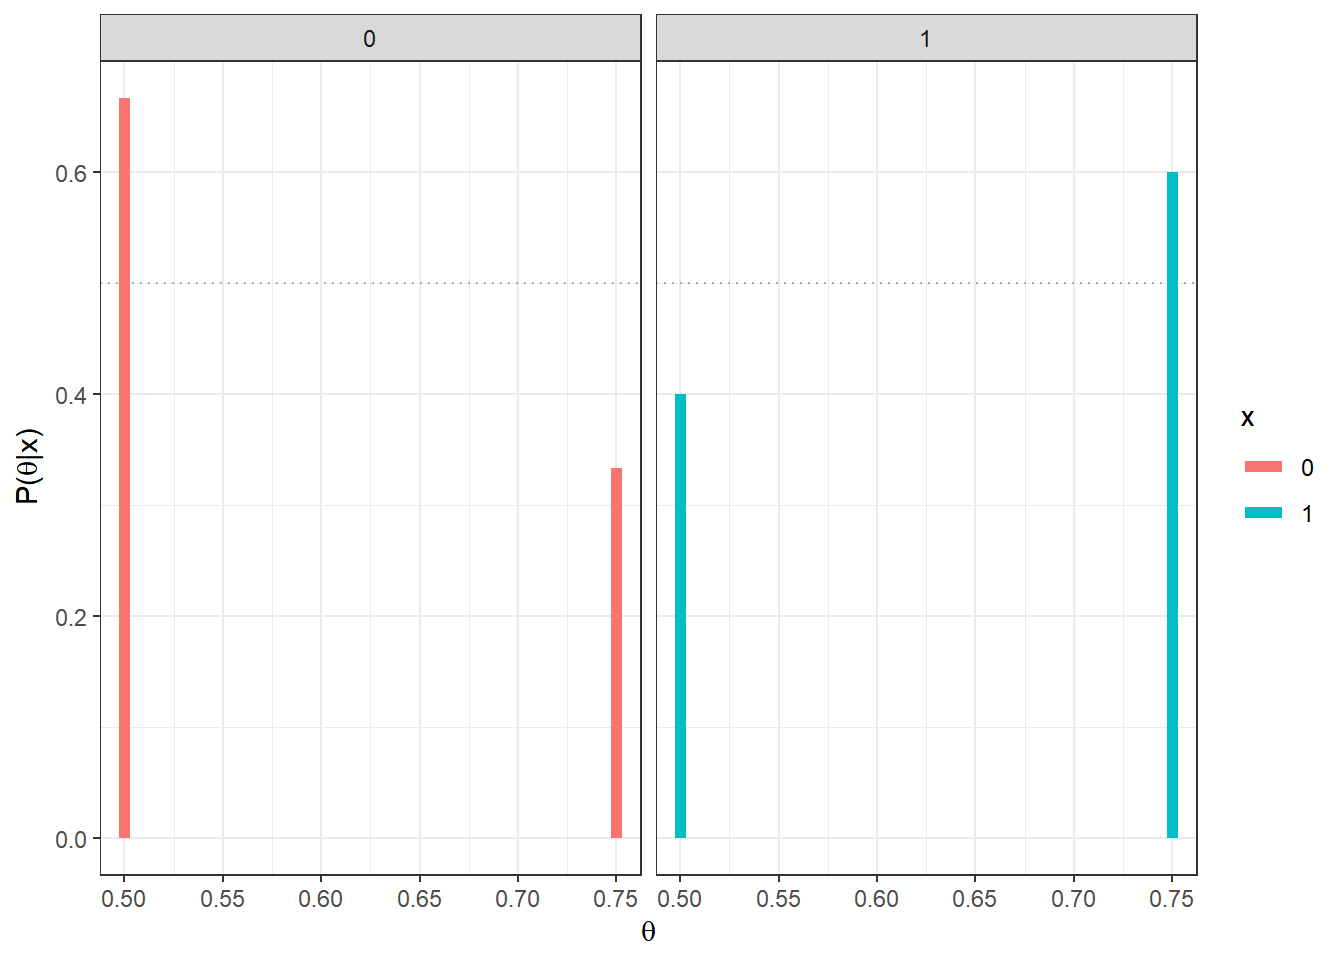
\includegraphics[width=0.7\linewidth]{InfBayes_files/figure-latex/unnamed-chunk-2-1} \end{center}

Assim, se sua decisão for escolher o valor mais provável de \(\theta\) após observar \(x\), a conclusão seria que a moeda é viesada \((\theta=3/4)\) se for observado cara \((x=1)\) e que a moeda é honesta \((\theta=1/2)\) se o resultado for coroa \((x=0)\).

\(~\)

\textbf{Exemplo 1.b:} Considere agora que serão realizados \(n\) lançamentos da moeda, de modo que agora tem-se \(X|\theta \sim Bin(n,\theta)\), \(\theta \in \{1/2,3/4\}\), \(x \in \{0,1,\ldots,n\}\). Suponha que observa-se \(X=x\).

\(f(\theta=3/4|X=x)\) \(=\dfrac{f(x|\theta=3/4)f(\theta=3/4)}{\displaystyle \sum_{\theta\in \{1/2,3/4\}}f(x|\theta)f(\theta)}\) \(=\dfrac{\displaystyle \binom{n}{x}\left(\dfrac{3}{4}\right)^x\left(\dfrac{1}{4}\right)^{n-x}\dfrac{1}{2}}{\displaystyle \binom{n}{x}\left(\dfrac{3}{4}\right)^x\left(\dfrac{1}{4}\right)^{n-x}\dfrac{1}{2}+\displaystyle\binom{n}{x}\left(\dfrac{1}{2}\right)^x\left(\dfrac{1}{2}\right)^{n-x}\dfrac{1}{2}}\) \(=\dfrac{1}{1+\left(\dfrac{2^n}{3^x}\right)}\) \(=\dfrac{3^x}{3^x + 2^n}\).

\begin{center}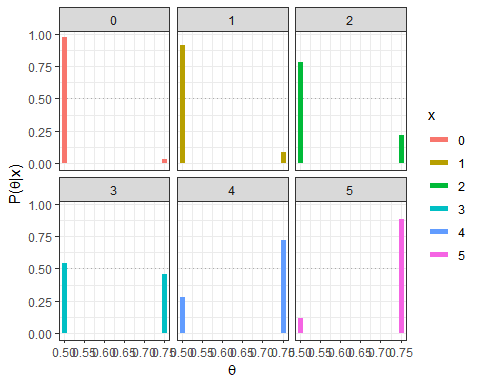
\includegraphics[width=0.7\linewidth]{InfBayes_files/figure-latex/unnamed-chunk-4-1} \end{center}

\(~\)

Note que o Exemplo 1.a é um caso particular desse exemplo quando \(n=1\). Se novamente sua decisão é baseada no valor mais provável de \(\theta\), temos

\(f(\theta=3/4|X=x) > \dfrac{1}{2}\) \(\Longleftrightarrow \dfrac{3^x}{3^x + 2^n} > \dfrac{1}{2}\) \(\Longleftrightarrow {3^x} > {2^n}\) \(\Longleftrightarrow \dfrac{x}{n} = \bar{x} > \log_3{2}\approx 0,63\).

\(~\)

\textbf{Exemplo 1.c:} Considere uma moeda será lançada \(n\) vezes mas que \(\theta\) é desconhecido, de modo que \(\Theta = [0,1]\). Para simplificar, vamos assumir \(f(\theta)=\mathbb{I}_{[0,1]}(\theta)\), isto é, \(\theta \sim Unif(0,1)\sim Beta(1,1)\). Essa priori corresponde ao caso onde você acredita que todos os valores possíveis para \(\theta\) são igualmente ``prováveis'', assim como nos exemplos anteriores. Novamente, \(X|\theta \sim Bin(n,\theta)\)

\(f(\theta|x)=\) \(\dfrac{f(x|\theta)f(\theta)}{\int_0^1 f(x|\theta)f(\theta)d\theta}=\) \(\dfrac{\binom{n}{x}\theta^x(1-\theta)^{n-x} ~~\mathbb{I}_{[0,1]}(\theta)}{\int_0^1\binom{n}{x}\theta^x(1-\theta)^{n-x}d\theta}=\) \(\dfrac{\dfrac{\Gamma(1+x+1+n-x)}{\Gamma(1+x)\Gamma(1+n-x)}~~\theta^x(1-\theta)^{n-x}~~\mathbb{I}_{[0,1]}(\theta)}{\underbrace{\displaystyle \int_0^1\dfrac{\Gamma(1+x+1+n-x)}{\Gamma(1+x)\Gamma(1+n-x)}~~\theta^x(1-\theta)^{n-x}d\theta}_{1}}\) \(=\dfrac{\Gamma(1+x+1+n-x)}{\Gamma(1+x)\Gamma(1+n-x)}~~\theta^x(1-\theta)^{n-x}~~\mathbb{I}_{[0,1]}(\theta)\).

\(~\)

Logo \(\theta|x \sim Beta(1+x,1+n-x)\). Nesse exemplo, o valor ``mais provável'' (com maior densidade a posteriori) para \(\theta\) é a moda da distribuição, \(Moda(\theta|x)\) \(= \dfrac{(1+x)-1}{(1+x)+(1+n-x)-2}\) \(= \dfrac{x}{n}\) \(=\bar{x}\).

\(~\)

\textbf{Exemplo 1.d} Por fim, suponha que no exemplo anterior, sua opinião a priori é representada por uma distribuição beta qualquer com parâmetros \(a\) e \(b\), \(a,b > 0\). Desta forma, \(X|\theta \sim Bin(n,\theta)\) e \(\theta\sim Beta(a,b)\). Calculando a distribuição a posteriori de forma similar ao exemplo anterior, temos que \(\theta|X=x \sim Beta(a+x,b+n-x)\).

\(~\)

\begin{center}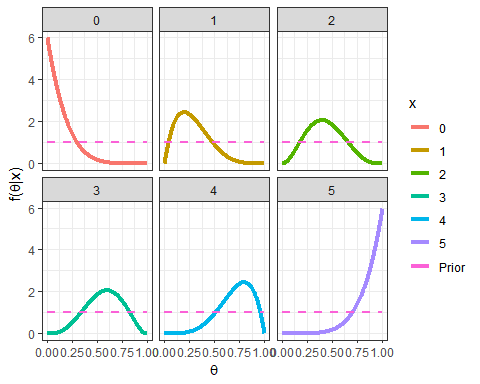
\includegraphics[width=0.7\linewidth]{InfBayes_files/figure-latex/unnamed-chunk-6-1} \end{center}

\(~\)

Suponha que \(a=b=1\) (como no exemplo anterior), \(n=5\) e \(x=2\), de modo que \(\theta|x=2 \sim Beta(3,4)\). Algumas medidas resumo da distribuição posterior para esse exemplo são

\begin{itemize}
\item
  \(Moda(\theta|x)\) \(=\dfrac{a+x-1}{a+b+n-2}\) \(=\dfrac{2}{5}\) \(=0,4\);
\item
  \(E[\theta|x]\) \(=\dfrac{a+x}{a+b+n}\) \(=\dfrac{3}{7}\) \(=0,43\);
\item
  \(Med(\theta|x)\) \(\approx \dfrac{a+x-1/3}{a+b+n-2/3}\) \(=\dfrac{8/3}{19/3}\) \(\approx 0,42\);
\item
  \(Var(\theta|x)\) \(=\dfrac{(a+x)(b+n-x)}{(a+b+n)^2(a+b+n+1)}\) \(=\dfrac{12}{392}\) \(\approx 0,031\).
\end{itemize}

\(~\)

\hypertarget{distribuiuxe7uxe3o-a-priori}{%
\section{Distribuição a Priori}\label{distribuiuxe7uxe3o-a-priori}}

\begin{itemize}
\tightlist
\item
  A priori é sempre subjetiva (assim como a escolha do modelo estatístico)!

  \begin{itemize}
  \tightlist
  \item
    Por exemplo, dizer que os dados seguem uma distribuição normal, é uma escolha subjetiva, muitas vezes baeadas nas facilidades mathemáticas que essa distribuição proporciona.\\
  \item
    Do mesmo modo, suponha que dois indivíduos que consideram que a distribuição do parêmetro é simétrica, com mesmas suposições sobre média e variância. O primeiro pode optar por representar sua distribuição usando uma distribuição Normal, enquanto o segundo pode utilizar uma distribuição T ou Cauchy.\\
  \end{itemize}
\item
  Não existe ``opinião errada'', existem opiniões diferentes, dado o nível de conhecimento e as experiências prévias do indivíduo.\\
\item
  A priori deve ser sua opinião apenas sobre o parâmetro \(\theta\) e não deve depender de fatores como o desenho do experimento ou o objetivo do estudo.
\end{itemize}

\hypertarget{prioris-baseada-na-opiniuxe3o-de-um-especialista}{%
\subsection{Prioris Baseada na Opinião de um Especialista}\label{prioris-baseada-na-opiniuxe3o-de-um-especialista}}

\hypertarget{muxe9todo-do-histograma}{%
\subsubsection{Método do Histograma}\label{muxe9todo-do-histograma}}

\begin{itemize}
\item
  Muitas vezes, para ``extrair'' o conhecimento de um especialista, podemos dividir o espaço paramétrico em regiões e pedir para o especialista ``ordenar'' esses conjuntos, utilizando ``pesos'' que refletem a crença que o parâmetro esteja em cada uma daquelas regiões.
\item
  \textbf{Exemplo 1.} (\emph{Bayesian Computation with R}, Albert,J., pág 27)

  \begin{itemize}
  \tightlist
  \item
    Seja \(\theta\) uma proporção desconhecida \((\Theta=[0,1])\);\\
  \item
    Considere a partição \(T = \left\{[0,0.1), [0.1,0.2), \ldots, [0.9,1] \right\}\);
  \item
    Suponha que um especialistas atribui pesos \(p=(1, 5.2, 8, 7.2, 4.6, 2.1, 0.7, 0.1, 0, 0)\) a esse intervalos;\\
  \item
    A piori, nesse caso, é o histograma apresentado a seguir.
  \end{itemize}
\end{itemize}

\begin{center}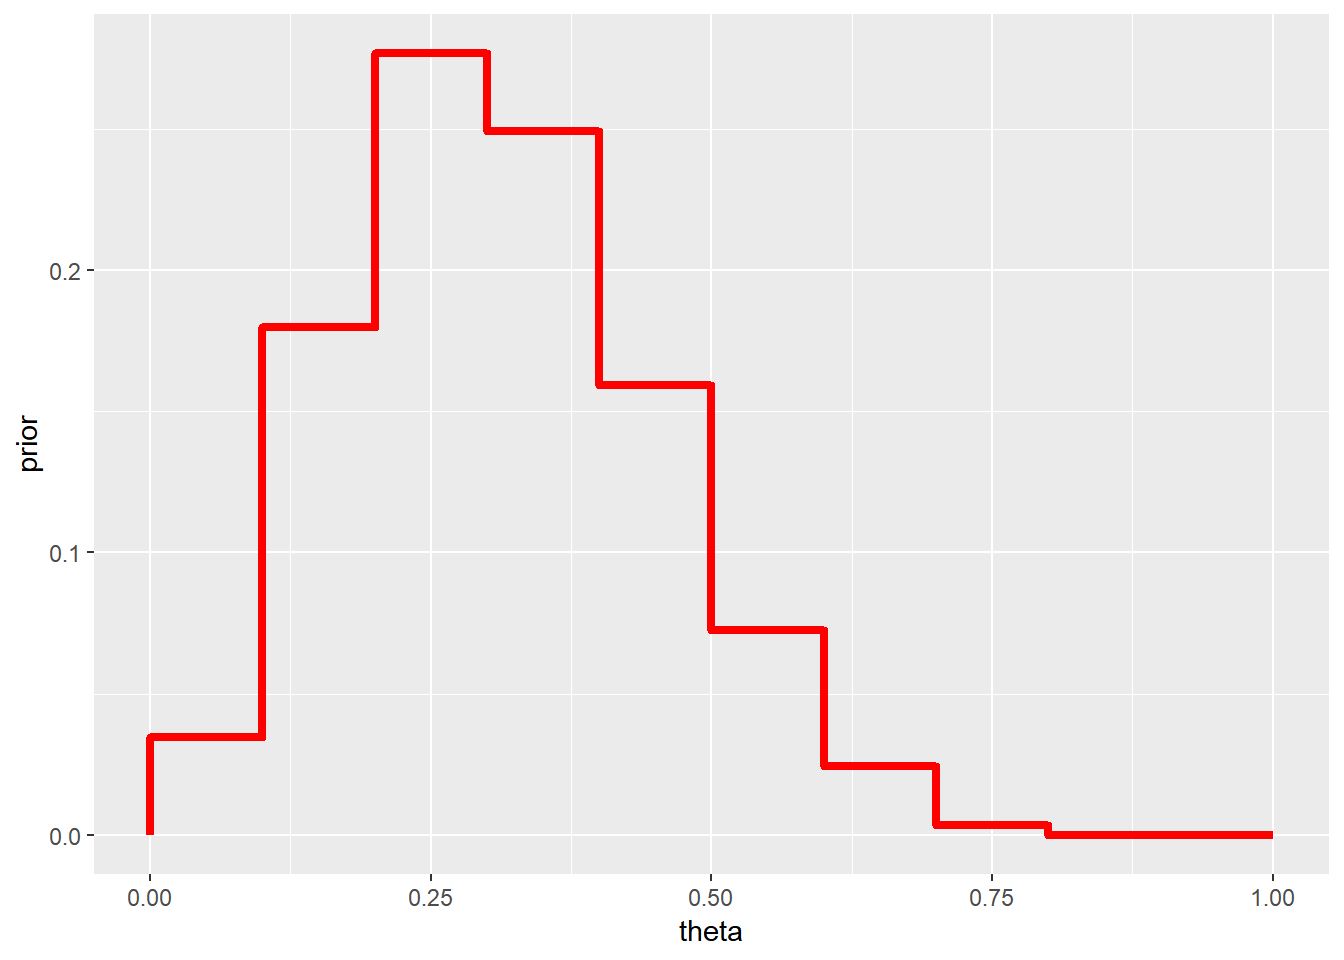
\includegraphics[width=0.7\linewidth]{InfBayes_files/figure-latex/unnamed-chunk-8-1} \end{center}

\begin{itemize}
\tightlist
\item
  Voltando ao exemplo da moeda, suponha novamente que foram observados \(x=2\) sucessos em \(n=5\) lançamentos. A posteriori nesse caso pode ser obtida multiplicando a distribuição a priori pela verossimilhança e ``padronizando'' a função obtida. Assim:
\end{itemize}

\begin{center}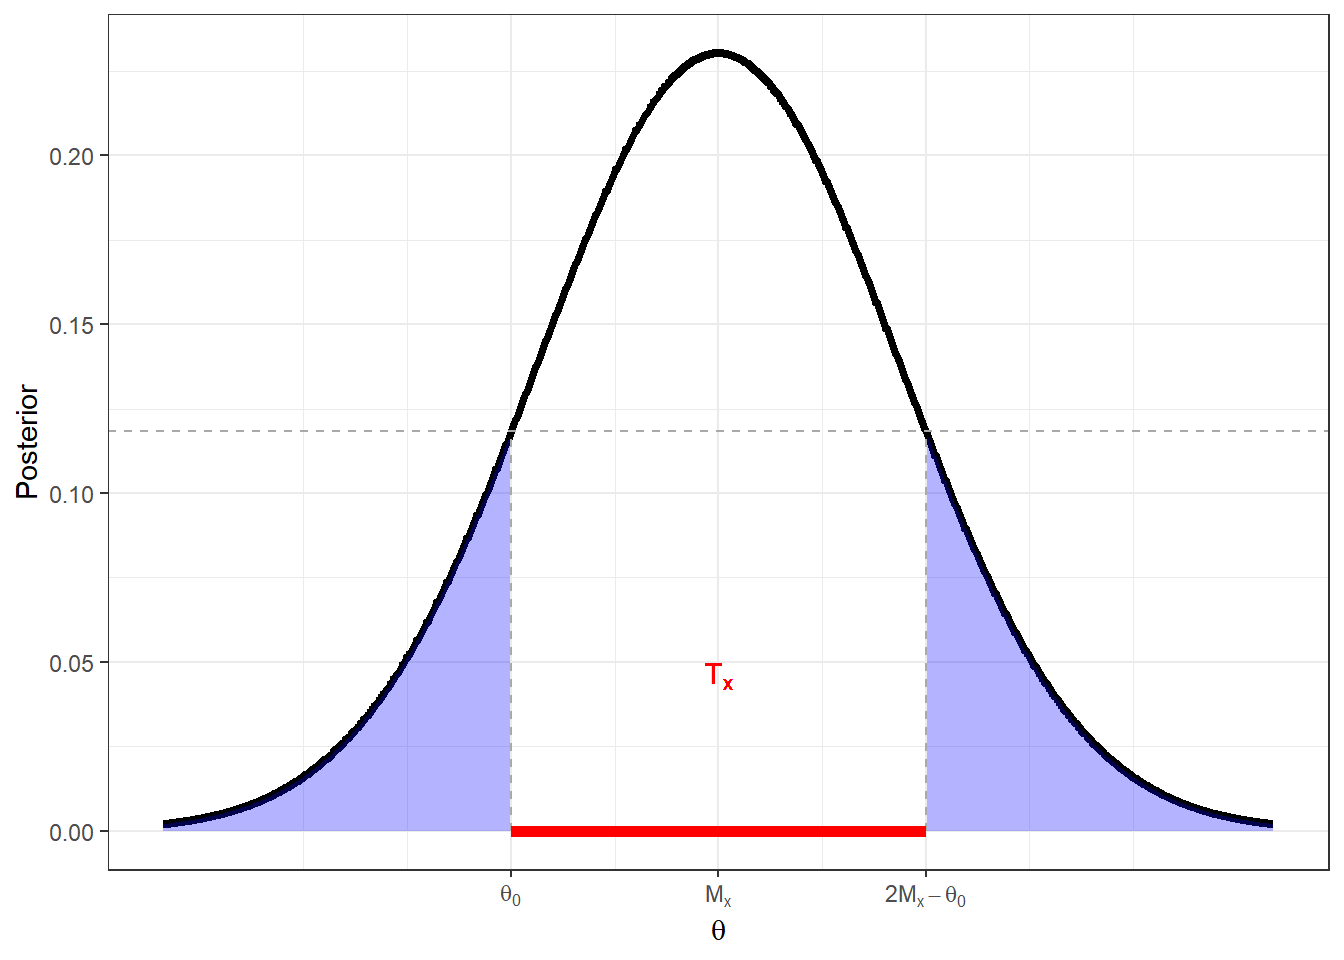
\includegraphics[width=0.7\linewidth]{InfBayes_files/figure-latex/unnamed-chunk-9-1} \end{center}

\(~\)

\hypertarget{elicitauxe7uxe3o-de-hiperparuxe2metros}{%
\subsubsection{Elicitação de Hiperparâmetros}\label{elicitauxe7uxe3o-de-hiperparuxe2metros}}

\begin{itemize}
\tightlist
\item
  Nessa abordagem, a priori é obtida da seguinte maneira:

  \begin{enumerate}
  \def\labelenumi{\arabic{enumi}.}
  \tightlist
  \item
    Escolha uma família de distribuições conveniente. O conceito de ``conveniência'' aqui pode levar em conta, por exemplo, o suporte da distribuição, se é flexível o suficiente para acomodar diversos tipos de opinião, se permite a obtenção analítica da posteriori e assim por diante;\\
  \item
    Obtenha um conjunto de medidas resumo (como média, variância, quantis, etc.);\\
  \item
    Utilize as medidas resumo para calcular hiperparâmetros da distribuição escolhida.
  \end{enumerate}
\end{itemize}

\(~\)

\begin{itemize}
\item
  \textbf{Exemplo:} Na seção anterior, a priori dada pelo histograma tem média \(m=0.31\) e variância aproximadamente \(v=0.02\). Podemos utilizar como priori, por exemplo, uma distribuiçaõ beta com essa média e variância, já que a beta tem um suporte conveniente e facilita as contas, como também já vimos. Assim, vamos considerar uma distribuição \(Beta(a,b)\) e escolher \(a\) e \(b\) satisfazendo:

  \begin{enumerate}
  \def\labelenumi{(\roman{enumi})}
  \tightlist
  \item
    \(E[\theta]\) \(=\dfrac{a}{a+b}\) \(=m\) \(\Longleftrightarrow b=\left(\dfrac{1-m}{m}\right)a\)
  \item
    \(Var(\theta)\) \(=\dfrac{ab}{(a+b)^2(a+b+1)}\) \(=0.02\) \(\Longleftrightarrow a=\dfrac{m(m-m^2-v)}{v}\)
  \end{enumerate}
\end{itemize}

Resolvendo o sistema temos, de forma geral, que \(a=\dfrac{m(m-m^2-v)}{v}\) e \(b=\dfrac{(1-m)(m-m^2-v)}{v}\).

Assim, no nosso exemplo, teríamos uma \(Beta(3,6.7)\). Além disso, já vimos que, nesse caso, a distribuição a posteriori é \(Beta(3+x,6.7+n-x)\). Considerando novamente \(n=5\) e \(x=2\), temos:

\begin{center}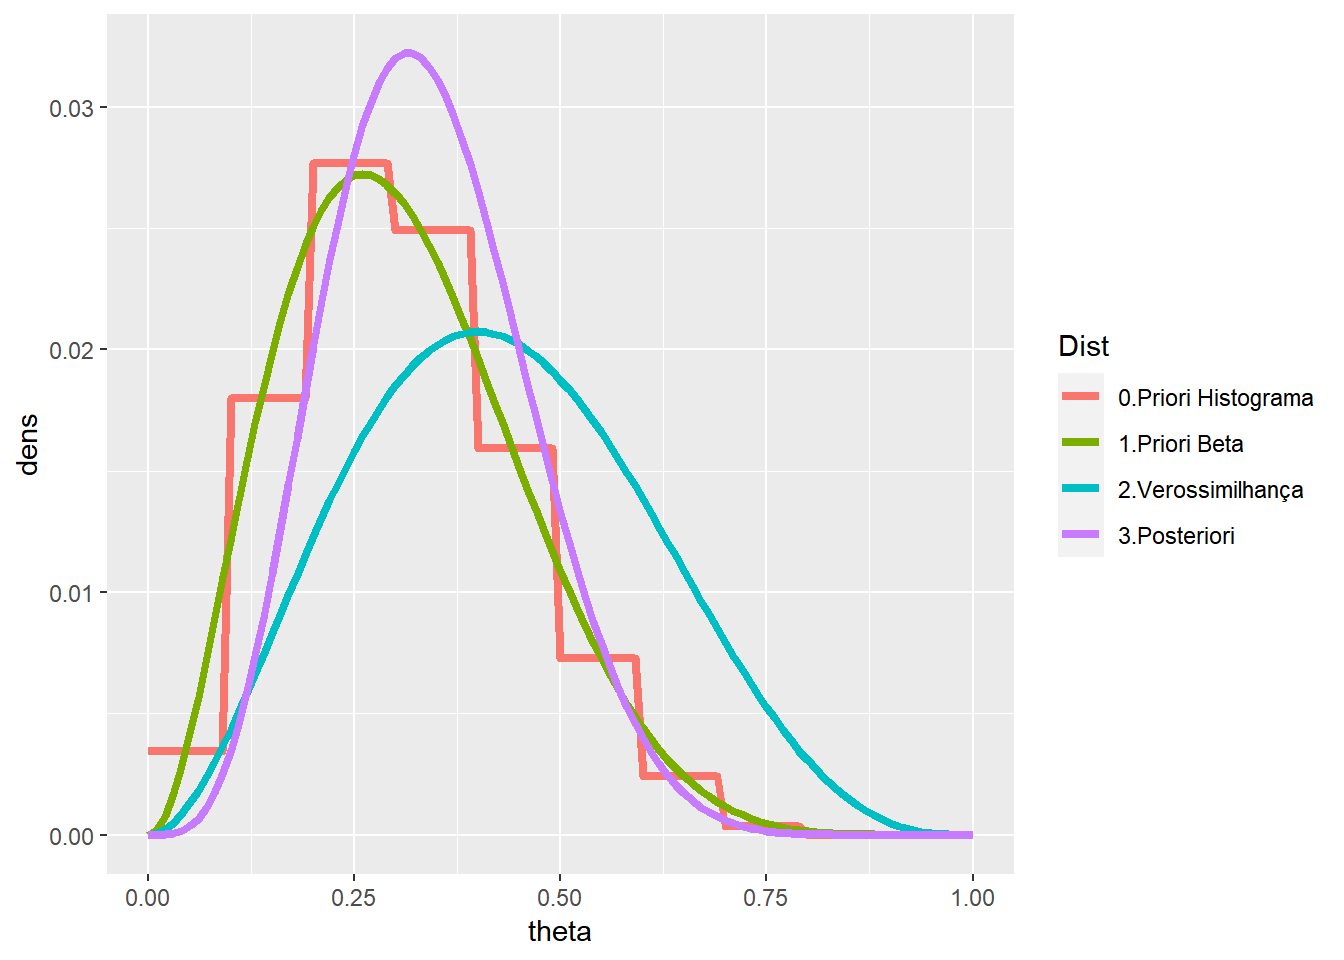
\includegraphics[width=0.7\linewidth]{InfBayes_files/figure-latex/unnamed-chunk-10-1} \end{center}

\(~\)

\hypertarget{prioris-conjugadas}{%
\subsection{Prioris Conjugadas}\label{prioris-conjugadas}}

Como visto no exemplo da moeda, quando distribuição a priori era \(Beta(a,b)\), a posteriori era facilmente obtida e também estava na classe das distribuições \(Beta\). Em particular, quando observa-se \(x\) sucessos em \(n\) realizações de ensaios de Bernoulli, a distribuição a posteriori é \(Beta(a+x,b+n-x)\). Isso ocorre pois essa distribuição pertence à uma classe bastante espefícica de distribuições a priori, chamadas distribuições conjugadas.

\(~\)

\textbf{Definição} Seja \(\mathcal{P}=\{f(x|\theta):\;\theta \in \Theta\}\) uma família de distribuições (condicionais) para \(\boldsymbol{X}\) e considere \(\mathcal{C}=\{h(\theta|a):\;a\in A\}\) uma família de distribuições para \(\theta\). Dizemos que (a família) \(\mathcal{C}\) é \textbf{conjugada} para \(\mathcal{P}\) se, \(\forall \;h(\theta)\in \mathcal{C},\) \(h(\theta|\boldsymbol{x})\propto f(\boldsymbol x|\theta)h(\theta) \in \mathcal{C},\forall \boldsymbol x \in \mathfrak{X}.\)

\(~\)

\textbf{Resultado 1.} Seja \(X\) v.a. tal que, condicional ao conhecimento de \(\theta,\) \(X|\theta \sim Bin(n,\theta).\) Considere que, a priori, \(\theta \sim Beta(a,b).\) Então, \(\theta|X=x \sim Beta(a+x,b+n-x).\) Por tanto, a família \(\mathcal{C}=\{Beta(a_1,a_2):\;(a_1,a_2)\in \mathbb{R}^2_+\}\) é conjugada para \(\mathcal{P}=\{Bin(n,\theta):\;\theta \in [0,1]\}.\)

\(~\)

\begin{itemize}
\tightlist
\item
  Esse resultado também vale se

  \begin{enumerate}
  \def\labelenumi{\arabic{enumi}.}
  \tightlist
  \item
    \(X_1,...,X_n\) são v.a.s \emph{condicionalmente independentes e identicamente distribuidas} (c.i.i.d.) com \(X_i|\theta \sim Ber(\theta)\)\\
  \item
    \(X_i|\theta\sim Geo(\theta),\) \(i=1,...,n \; c.i.i.d.\)\\
  \item
    \(X_i|\theta \sim BinNeg(k,\theta)\)\\
    \(\theta\sim Beta(a,b)\Rightarrow\) \(\theta|\boldsymbol X=\boldsymbol x \sim Beta(a+s,b+f)\) onde \(s\) é o número de sucessos e \(f\) é o número de fracassos.
  \end{enumerate}
\end{itemize}

\(~\)

\textbf{Resultado 2.} (\emph{generalização do resultado anterior para o caso onde o número de categorias é maior que 2})

Seja \(\boldsymbol X | \boldsymbol \theta \sim Multinomial(n,\boldsymbol \theta)\), isto é, sua função de probabilidade é dada por

\[f(\boldsymbol x| \boldsymbol \theta)= \binom{n}{x_1,x_2,...,x_k}~\prod_{i=1}^{k-1}\theta^i~\underbrace{\left(1-\sum_{i=1}^{k-1}\theta_i\right)^{\displaystyle n-\sum_{i=1}^{k-1}x_i}}_{\displaystyle \theta_k^{~~x_k}}\]

onde \(\theta_i\in [0,1]\) com \(\sum_{i=1}^K\theta_i=1\), \(x_i \in \{0,1,...,n\}\) com \(\sum_{i=1}^nx_i=n\) e \(\displaystyle \binom{n}{x_1,x_2,...,x_k}=\dfrac{n!}{x_1!x_2!...x_k!}\).

Considere que, a priori, \(\boldsymbol \theta \sim Dirichlet(a_1,...,a_k),\) \(a_i > 0, i=1,...,k\), isto é, a f.d.p. a priori para \(\boldsymbol \theta\) é dada por

\[f(\boldsymbol \theta) = \dfrac{\Gamma(\sum_{i=1}^K a_i)}{\Gamma(a_1)\Gamma(a_2)...\Gamma(a_k)}\prod_{i=1}^{k-1}\theta_i^{a_i-1}\bigg(\underbrace{1-\sum_{i=1}^{k-1}\theta_i}_{\theta_k}\bigg)^{a_k-1}.\]

Então, a distribuição a posteriori para \(\boldsymbol \theta\) é
\(\boldsymbol \theta|\boldsymbol X = \boldsymbol x \sim Dirichlet (a_1+x_1,...,a_k+x_k)\).

\(~\)

\begin{quote}
\textbf{Demo:} Para verificar o resultado, basta ver que\\
\(f(\boldsymbol\theta|\boldsymbol x)\) \(=\dfrac{f(\boldsymbol x| \boldsymbol \theta)f(\boldsymbol \theta)}{\int_\Theta f(\boldsymbol x| \boldsymbol \theta)f(\boldsymbol \theta)d\boldsymbol \theta}\) \(\propto f(\boldsymbol x| \boldsymbol \theta)f(\boldsymbol \theta)\) \(\propto \prod_{i=1}^{k-1}\theta_i^{(a_i+x_i-1)}\left(1-\sum_{i=1}^{k-1}\theta_i\right)^{(a_k+x_k)-1}\)
\end{quote}

\(~\)

\textbf{Resultado 3.} seja \(X_1,...,X_n\) v.a. c.i.i.d tais que \(X_i|\theta \sim Unif(0,\theta)\) e considere que, a priori,\(\theta \sim Pareto(a,b)\). Então \(\theta|\boldsymbol X = \boldsymbol x \sim Pareto\left(a+n,max\{b,x_{(n)}\}\right)\).

\(~\)

\begin{quote}
\textbf{Demo:}\\
\(f(\boldsymbol x|\theta)\) \(\overset{ci}{=}\prod_{i=1}^nf(x_i|\theta)\) \(\overset{id}{=}\prod_{i=1}^n\dfrac{1}{\theta}\mathbb{I}_{[0,\theta]}(x_i)\) \(=\dfrac{1}{\theta^n}\mathbb{I}_{[0,\theta]}(x_{(n)})\) \(=\dfrac{1}{\theta^n}\mathbb{I}_{[x_{(n)},+\infty)}(\theta)\)\\
onde \(x_{(n)}=max\{x_1,...,x_n\}\).\\
\(~\)\\
\(f(\theta)=\dfrac{ab^a}{\theta^{a+1}}\mathbb{I}_{[b,+\infty]}(\theta)\).\\
Então\\
\(f(\theta| \boldsymbol x)\) \(\propto f(\boldsymbol x|\theta)f(\theta)\) \(=\dfrac{1}{\theta^{a+n+1}}\mathbb{I}_{[x_{(n)},+\infty)}(\theta)\mathbb{I}_{[b,+\infty)}(\theta)\) \(=\dfrac{1}{\theta^{a+n+1}}\mathbb{I}_{[max\{b,x_{(n)}\},+\infty)}(\theta)\)\\
\(~\)
\(\Rightarrow \theta|\boldsymbol X = \boldsymbol x \sim Pareto(a+n,max\{b,x_{(n)}\})\).
\end{quote}

\(~\)

\textbf{Resultado 4.} Seja \(X_1,...,X_n,Y_1,...,Y_m\) v.a. condicionalmente independentes tais que \(X_i|\theta\sim Exp(\theta),i=1,...,n\) e \(Y_j|\theta \sim Poisson(\theta),j=1,...,m\). Considere que, a priori, \(\theta \sim Gama(a,b)\). Então \(\theta| \boldsymbol x,\boldsymbol y \sim Gama(a+n+\sum_jy_j~,~b+m+\sum_ix_i)\).

\begin{quote}
\textbf{Demo:}\\
\(f(\boldsymbol x, \boldsymbol y|\theta)\overset{ci}{=}f(\boldsymbol x|\theta)f(\boldsymbol y|\theta)\overset{ci}{=}\) \(\prod_{i=1}^nf(x_i|\theta)\prod_{j=1}^mf(y_i|\theta)=\) \(\prod_{i=1}^n\theta e^{-\theta x_i}\prod_{j=1}^m\dfrac{\theta^{y_j}e^{-\theta}}{y_j!}=\) \(\dfrac{1}{\prod_{j=1}^my_j!}\theta^{n+\sum_j y_j}e^{-(m+\sum_ix_i)\theta}\)\\
\(~\)\\
\(f(\theta)=\dfrac{b^a}{\Gamma(a)}\theta^{a-1}e^{-b\theta}\)
\(~\)\\
\(f(\theta| \boldsymbol{x,y})\propto f(\boldsymbol x, \boldsymbol y|\theta)f(\theta)\propto\) \(\theta^{[a+n+\sum_jy_j]-1}e^{-[b+m+\sum_ix_i]\theta}\)
\(~\)\\
\(\Rightarrow \theta| \boldsymbol x,\boldsymbol y \sim Gama(a+n+\sum_jy_j,b+m+\sum_ix_i)\)
\end{quote}

\(~\)

\textbf{Resultado 5.} Seja \(~\mathcal{P}=\{f(\boldsymbol x|\theta):\; \theta \in \Theta\}~\) e \(~\mathcal{C}=\{h(\theta|a):\;a\in A\}~\) uma \emph{família conjugada} para \(\mathcal{P}\). Considere \(\mathcal{M}=\{h(\theta)=\sum_{i=1}^mw_ih_i(\theta):\) \(h_i \in \mathcal{C} \; e \; w_i>0,\; \sum_{i=1}^m w_i=1\}\). Então \(\mathcal{M}\) é \emph{família conjugada} para \(\mathcal{P}\).

\begin{quote}
\textbf{Demo:} Como \(\mathcal{C}\) é conjugada para \(\mathcal{P}\), para toda função \(h_i \in \mathcal{C}\), temos que \(f_i(\theta|\boldsymbol x)\propto h_i(\theta)f(\boldsymbol x|\theta)\in \mathcal{C}\). Então\\
\(~\)\\
\(h\in \mathcal{M}\) \(~\Rightarrow~ f(\theta|\boldsymbol x)\) \(~\propto~ h(\theta)f(\boldsymbol x|\theta)\) \(~\propto~\sum_{i=1}^m w_i\underbrace{h_i(\theta)f(\boldsymbol x|\theta)}_{\in \mathcal{C}}\) \(~\propto~\sum_{i=1}^m w_i^*f_i(\theta|\boldsymbol x)\in \mathcal{M}\).
\end{quote}

\(~\)

\textbf{Exemplo.} Seja \(X|\theta \sim Bin(n,\theta)\) e \(f(\theta)\) \(=wf_1(\theta)+(1-w)f_2(\theta)\), onde \(f_1\sim Beta(a_1,b_1)\) e \(f_2\sim Beta(a_2,b_2)\).

\(~\)

\(f(\theta|x)\) \(=\dfrac{f(x|\theta)f(\theta)}{\int_0^1f(x|\theta)f(\theta)}\) \(=\dfrac{f(x|\theta)[wf_1(\theta)+(1-w)f_2(\theta)]}{w\int_0^1f_1(\theta)f(x|\theta)d\theta+(1-w)\int_0^1f_2(\theta)d\theta}\)

\(\propto\dfrac{w\binom{n}{x}\frac{\Gamma(a_1+b_1)}{\Gamma(a_1)\Gamma(b_1)}\theta^{a_1+x-1}(1-\theta)^{b_1+n-x-1}+(1-w)\binom{n}{x}\frac{\Gamma(a_2+b_2)}{\Gamma(a_2)\Gamma(b_2)}\theta^{a_2+x-1}(1-\theta)^{b_2+n-x-1}}{\underbrace{w\binom{n}{x}\frac{\Gamma(a_1+b_1)}{\Gamma(a_1)\Gamma(b_1)}\frac{\Gamma(a_1+x)\Gamma(b_1+n-x)}{\Gamma(a_1+b_1+n)}}_{A}+\underbrace{(1-w)\binom{n}{x}\frac{\Gamma(a_2+b_2)}{\Gamma(a_2)\Gamma(b_2)}\frac{\Gamma(a_2+x)\Gamma(b_2+n-x)}{\Gamma(a_2+b_2+n)}}_{B}}\)

\(\propto~\underbrace{\dfrac{A}{A+B}}_{w^*}Beta(a_1+x,b_1+n-x)+\underbrace{\dfrac{B}{A+B}}_{1-w^*}Beta(a_2+x,b_2+n-x)\)

\(~\)

Primeiramente, suponha que \(n=5\), e temos uma mistura das distribuições \(Beta(5,12)\) e \(Beta(10,3)\), com \(w=0.5\). O gráfico a seguir apresenta as distribuições a priori, a verossimilhança e a posteriori para cada possível valor de \(x\) em \(\left\{0,1,\ldots,5\right\}\).

\begin{center}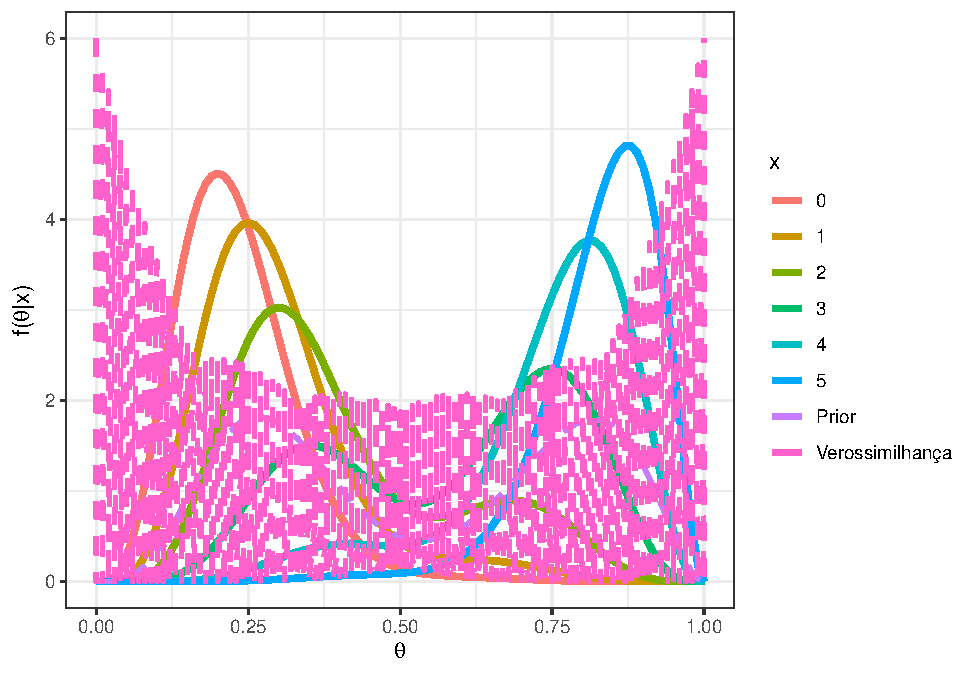
\includegraphics[width=0.7\linewidth]{InfBayes_files/figure-latex/unnamed-chunk-11-1} \end{center}

\(~\)

Agora, suponha que \(n=5\) e foi observado \(x=2\). Novamente, considere a mistura das distribuições \(Beta(5,12)\) e \(Beta(10,3)\) mas agora com pesos \(w\) variando no conjunto \(\left\{0,0.1,\ldots,0.9,1\right\}\).

\begin{center}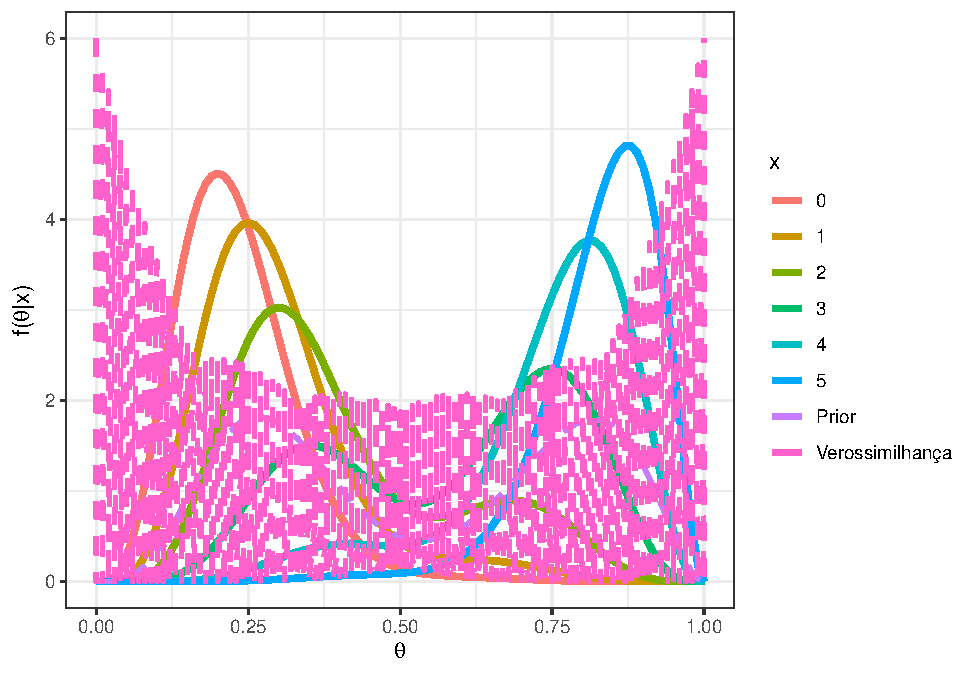
\includegraphics[width=0.7\linewidth]{InfBayes_files/figure-latex/unnamed-chunk-13-1} \end{center}

\(~\)

\hypertarget{ape}{%
\chapter{Apendice: Breve Resumo de Medida e Probabilidade}\label{ape}}

\hypertarget{breve-resumo-de-medida-e-probabilidade}{%
\section{Breve Resumo de Medida e Probabilidade}\label{breve-resumo-de-medida-e-probabilidade}}

\begin{itemize}
\item
  \(\Omega\): espaço amostral (um conjunto não vazio).
\item
  \(\mathcal{A}\): \emph{\(\sigma\)-álgebra de subconjuntos} de \(\Omega\), isto é,

  \begin{enumerate}
  \def\labelenumi{\arabic{enumi}.}
  \tightlist
  \item
    \(\Omega \in \mathcal{A}\);
  \item
    \(A \in \mathcal{A} \Longrightarrow A^{c} \in \mathcal{A}\);
  \item
    \(\displaystyle A_1, A_2, \ldots \in \mathcal{A} \Longrightarrow \bigcup_{i\geq1} A_i \in \mathcal{A}\).
  \end{enumerate}
\item
  Os elementos de \(\mathcal{A}\) são chamados de \emph{eventos} e serão denotados por \(A, B, C, \ldots, A_1, A_2, \ldots\)
\item
  \((\Omega, \mathcal{A})\): \emph{espaço mensurável}.
\item
  Usualmente, denota-se a \(\sigma\)-álgebra gerada por um conjunto \(\mathcal{C}\) como \(\sigma(\mathcal{C})\). Por exemplo:

  \begin{itemize}
  \tightlist
  \item
    \(\sigma(\Omega) = \{\emptyset,\Omega\}~~\) (\(\sigma\)-ágebra trivial);
  \item
    Para \(A \subset \Omega\), \(\sigma(A) = \{\emptyset, A, A^c, \Omega\}\);
  \item
    \(\sigma(\mathbb{N}) = \mathcal{P}(\mathbb{N})~~\) (partes de \(\mathbb{N}\), todos o subconjuntos de \(\mathbb{N}\));
  \item
    \(\sigma\left(\left\{(-\infty,x): x \in \mathbb{R}\right\}\right) = \mathcal{B}\left(\mathbb{R}\right)~~\) (borelianos de \(\mathbb{R}\))
  \end{itemize}
\end{itemize}

\(~\)

\begin{itemize}
\tightlist
\item
  \(\mu: \mathcal{A} \longrightarrow \bar{\mathbb{R}}_+\) é uma \emph{medida} se

  \begin{enumerate}
  \def\labelenumi{\arabic{enumi}.}
  \tightlist
  \item
    \(\mu(\emptyset) = 0\);
  \item
    \(\displaystyle A_1, A_2, \ldots \in \mathcal{A}\) com \(A_i \bigcap A_j = \emptyset\) , \(\forall i \neq j\) , \(\displaystyle \mu\left(\bigcup_{i \geq 1} A_i\right) = \sum_{i \geq 1} \mu\left(A_i\right)\).
  \end{enumerate}
\item
  \((\Omega,\mathcal{A}, \mu)\) é chamado de \emph{espaço de medida}.
\end{itemize}

\(~\)

\begin{quote}
\textbf{Exemplo 1 (medida de contagem):} Seja \(\Omega\) um conjunto não vazio e \(A\subseteq \Omega\). Defina \(\mu(A)=|A|\) como o número de elementos (cardinalidade) de \(A\). Assim, \(\mu(\Omega) > 0\), \(\mu(\emptyset)=0\) e, se \((A_n)_{n \geq 1}\) é uma sequência de eventos disjuntos, então \(\mu(\cup A_n) = \sum \mu(A_n)\). Note que \(\mu(A)=\infty\) é possivel se \(\Omega\) tem infinitos elementos.
\end{quote}

\(~\)

\begin{quote}
\textbf{Exemplo 2 (medida de Lebesgue):} Seja \(\Omega=\mathbb{R}\) e \(A\subseteq \Omega\) um intervalo. Se \(A\) é limitado, defina \(\mu(A)\) como o comprimento do intervalo A. Se \(A\) não é limitado, \(\mu(A)=\infty\). Note que \(\mu(\mathbb{R})=\infty\), \(\mu(\emptyset)=0\) e, se \(A_1 \cap A_2 = \emptyset\) e \(A_1 \cup A_2\) é um intervalo (ou uma união de intervalos disjuntos), então \(\mu(A_1 \cup A_2) = \mu(A_1) + \mu(A_2)\).
\end{quote}

\(~\)

\begin{quote}
\textbf{Exemplo 3:} Seja \(f: \mathbb{R} \longrightarrow \mathbb{R}_+\) uma função contínua e não nula. Para cada intervalo \(A\), defina \(\displaystyle \mu(A) = \int_A f(x) dx = \int_{\mathbb{R}} \mathbb{I}_A(x) f(x) dx\). Então, \(\mu(\mathbb{R})>0\), \(\mu(\emptyset)=0\) e, se \(A_1 \cap A_2 = \emptyset\) e \(A_1 \cup A_2\) é um intervalo (ou uma união de intervalos disjuntos), então \(\mu(A_1 \cup A_2) = \mu(A_1) + \mu(A_2)\).
\end{quote}

\(~\)

\textbf{Definição:} Seja \((\Omega,\mathcal{A})\) um espaço mensurável e \(\mu_1\) e \(\mu_2\) medidas nesse espaço. Dizemos que \(\mu_2\) é \emph{absolutamente contínua} com relação à \(\mu_1\) se, \(\forall A \in \mathcal{A}\), \(\mu_1(A)=0\) \(~\Rightarrow~ \mu_2(A)=0\).

Nesse caso, dizemos que \(\mu_2\) é dominada por \(\mu_1\) ou que \(\mu_1\) é uma medida dominante para \(\mu_2\) e denotamos \(\mu_2 \ll \mu_1\).

\(~\)

\textbf{Teorema (de Radon-Nikodin):} Seja \(\mu_2 \ll \mu_1\) com \(\mu_1\) \(\sigma\)-finita. Então, \(\exists f: \Omega \longrightarrow [0,+\infty]\) tal que, \(\forall A \in \mathcal{A}\),
\[\mu_2(A) = \int_A f(x) d\mu_1(x).\]
Além disso, se \(g:\Omega \longrightarrow \mathbb{R}\) é \(\mu_2\)-integrável, então
\[\int g(x) d\mu_2(x) = \int g(x) f(x) d\mu_1(x).\]
A função \(f=\frac{d\mu_2}{d\mu_1}\) é chamada de derivada de Radon-Nikodin da medida \(\mu_2\) com relação à medida \(\mu_1\) e é única \(\mu_1\)-q.c.

\(~\)

\begin{itemize}
\item
  \(P: \mathcal{A} \longrightarrow [0,1]\) é uma \emph{medida de probabilidade} se

  \begin{enumerate}
  \def\labelenumi{\arabic{enumi}.}
  \tightlist
  \item
    \(P(\Omega) = 1\);
  \item
    \(\displaystyle A_1, A_2, \ldots \in \mathcal{A}\) com \(A_i \bigcap A_j = \emptyset\) , \(\displaystyle P\left(\bigcup_{i \geq 1} A_i\right) = \sum_{i \geq 1} P\left(A_i\right)\).
  \end{enumerate}
\item
  \((\Omega, \mathcal{A}, P)\): espaço de probabilidade
\item
  Seja \((\Omega,\mathcal{A})\) e \((\mathfrak{X},\mathcal{F})\) dois espaços mensuráveis. Se \(X: \Omega \longrightarrow \mathfrak{X}\) é chamado de \emph{quantidade aleatória} se uma função mensurável, isto é, se \(\forall B \in \mathcal{F}\), \(A = X^{-1}(B) \in \mathcal{A}\). Se \(\mathfrak{X} = \mathbb{R}\) e \(\mathcal{F}=\mathcal{B}\) (\(\sigma\)-álgebra de Borel), \(X\) é chamado \emph{variável aleatória}.
\item
  A medida de probabilidade induzida por \(X\) recebe o nome de \emph{distribuição de} \(X\):
  \[P_X(B) = P(\{\omega \in \Omega :  X(\omega) \in B\})\]
\end{itemize}

\begin{quote}
\textbf{Exemplo 1:} Seja \(\Omega=\mathfrak{X}=\mathbb{R}\) com a \(\sigma\)-álgebra de Borel e \(f\) uma função não negativa tal que \(\int f(x) dx = 1\). Defina \(\displaystyle\mu(A)= \int_A f(x) dx\) e \(X(\omega)=\omega\). Então, \(X\) é uma variável aleatória contínua com função de densidade de probabilidade (f.d.p.) \(f\) e \(\mu_x = \mu\). Além disso, \(\mu_X\) é absolutamente contínua com relação à medida de Lebesgue \((\mu_X \ll \lambda)\) e \(\frac{d\mu_X}{d\lambda}=f\).
\end{quote}

\(~\)

\begin{quote}
\textbf{Exemplo 2:} Seja \(\Omega=\mathbb{R}\) com a \(\sigma\)-álgebra de Borel, \(\mathfrak{X} = \{x_1,x_2,\ldots\}\) um conjunto enumerável. Seja \(f\) uma função não negativa definida em \(\mathfrak{X}\) tal que \(\displaystyle \sum_{i=1}^{\infty} f(x_1) = 1\). Defina \(\displaystyle \mu(A) = \sum_{\{i: x_i \in A\}} f(x_i)\). Então \(X\) é uma variável aleatória discreta com função de probabilidade (f.d.p.) \(f\) e \(\mu_X=\mu\). Além disso, \(\mu_X\) é absolutamente contínua com relação à medida de contagem \((\mu_X \ll \nu)\) e \(\frac{d\mu_X}{d\nu}=f\).
\end{quote}

\hypertarget{valor-esperado-de-x-ou-uma-ideia-da-tal-integral-de-lebesgue}{%
\section{\texorpdfstring{Valor Esperado de \(X\) (OU uma ideia da tal Integral de Lebesgue)}{Valor Esperado de X (OU uma ideia da tal Integral de Lebesgue)}}\label{valor-esperado-de-x-ou-uma-ideia-da-tal-integral-de-lebesgue}}

Por simplicidade, considere \(\Big(\Omega = [0,1]~,~~ \mathcal{A} = \mathcal{B}\left([0,1]\right)~,~~ P=\lambda\Big)\).

Considere uma variável aleatória discreta \(X: \Omega \longrightarrow \mathbb{R}\), assumindo valores em \(\mathfrak{X}=\{x_1,x_2,\ldots,x_k\}\) com probabilidades \(\{p_1,p_2,\ldots,p_k\}\) com \(x_i \geq 0, \forall i\). Já vimos que o \emph{valor esperado} (ou \emph{esperança}) de \(X\) é \(E[X] =\) \(\sum x_i P(X=x_i) =\) \(\sum x_i p_i\).

Podemos definir essa v.a. como

\(X(\omega) = \left\{\begin{array}{lccc} x_1, & 0 & \leq \omega \leq & p_1 \\  x_2, & p_1 & < \omega \leq & p_1+p_2 \\  \vdots & & & \\  x_j, & \sum_{i=1}^{j-1} p_j & < \omega \leq & \sum_{i=1}^{j} p_j \\  \vdots & & & \\  x_k, & 1-p_k & < \omega \leq& 1 \end{array}\right.\)

\begin{center}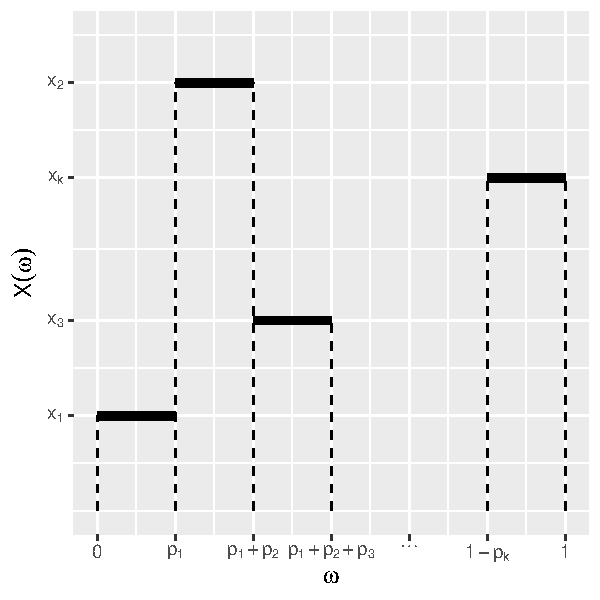
\includegraphics[width=0.7\linewidth]{InfBayes_files/figure-latex/va_discreta-1} \end{center}

Assim, temos que

\begin{itemize}
\item
  \(P_X(X=x_1) =\) \(P\left(\{\omega \in \Omega : X(\omega)=x_1\}\right) =\) \(\lambda\left([0,p_1]\right) =\) \(p_1\),
\item
  \(P_X(X=x_j) =\) \(P\left(\{\omega \in \Omega : X(\omega)=x_j\}\right) =\) \(\lambda\left(\left[\sum_{i=1}^{j-1} p_i,\sum_{i=1}^{j} p_i\right]\right) =\) \(p_j ~,~\) \(j \in \{2,\ldots,k\}\).
\end{itemize}

\(~\)

\textbf{Definição:} Uma função mensurável (v.a.) \(X: \Omega \longrightarrow \mathbb{R}_+\) é dita \emph{simples} se assumir um número finito de valores.

\(~\)

\textbf{Definição:} Considere \((\Omega, \mathcal{A}, P)\), \(X:\Omega\longrightarrow \mathbb{R}_+\) v.a. assumindo valores \(\{x_1,x_2,\ldots,x_k\}\) e \(A_1,A_2,\ldots,A_k\) eventos disjuntos em \(\mathcal{A}\). Seja \(\displaystyle X(\omega) = \sum_{i=1}^{k} x_i ~\mathbb{I}_{A_i}(\omega)\), uma função simples com \(A_i = X^{-1}(x_i)\), \(i=1,\ldots,k\). A \emph{integral de Lebesgue} de \(X\) em relação à medida \(P\) é
\[E[X] = \int_\Omega X dP = \sum_{i=1}^{k} x_i P(A_i).\]

\(~\)

\hypertarget{propriedades-da-integral-de-lebesque-de-x-v.a-em-relauxe7uxe3o-a-p}{%
\section{\texorpdfstring{Propriedades da integral (\emph{de Lebesque}) de \(X\) (v.a) em relação a \(P\)}{Propriedades da integral (de Lebesque) de X (v.a) em relação a P}}\label{propriedades-da-integral-de-lebesque-de-x-v.a-em-relauxe7uxe3o-a-p}}

\textbf{P1.} \(~\int_\Omega X dP \geq 0,\)

\textbf{P2.} \(~\int_\Omega cX dP = c\int_\Omega X dP.\)

\textbf{P3.} \(~\int_\Omega (X|Y) dP = \int_\Omega X dP + \int_\Omega Y dP\)

\(~\)

\begin{quote}
\textbf{Demo (P1):} Segue de \(x_i \geq 0\) e \(P(A_i) \geq 0\).
\end{quote}

\begin{quote}
\textbf{Demo (P2):}\\
Para \(X\) v.a. temos\\
\(X = \sum_{i=1}^kx_i~\mathbb{I}_{A_i}\) e \(cX\) (também v.a.)\\
\(cX = \sum_{i=1}^k(cx_i)~\mathbb{I}_{A_i}\), logo\\
\(\int_\Omega cX dP = \sum_{i=1}^k(cx_i) P(A_i)\) \(= c\sum_{i=1}^kx_i P(A_i) = c\int_\Omega X dP\)
\end{quote}

\begin{quote}
\textbf{Demo (P3):}\\
\(X = \sum_{i=1}^kx_i~\mathbb{I}_{A_i}\) e \(Y = \sum_{j=1}^ly_j~\mathbb{I}_{B_j}\).\\
\(\begin{array}{ll} X + Y & = \sum_{i=1}^k x_i ~\mathbb{I}_{A_i} + \sum_{j=1}^l y_j\\ & = \sum_{i=1}^k\sum_{j=1}^lx_i~\mathbb{I}_{A_i\cap B_j} + \sum_{i=1}^k\sum_{j=1}^ly_j~\mathbb{I}_{A_i\cap B_j}\\ \end{array}\)\\
\(\Longrightarrow X + Y = \sum_{i=1}^k\sum_{j=1}^l(x_i+y_j)~\mathbb{I}_{A_i\cap B_j}\).\\
\(\begin{array}{ll} \int_\Omega (X + Y) dP & = \sum_{i=1}^k\sum_{j=1}^l (x_i + y_j)P(A_i\cap B_j)\\ & = \sum_{i=1}^k\sum_{j=1}^l (x_i)P(A_i\cap B_j) + \sum_{i=1}^k\sum_{j=1}^l (y_j)P(A_i\cap B_j)\\ & = \sum_{i=1}^k x_i P(A_i) + \sum_{j=1}^l y_j P(B_j)\\ & = \int_\Omega X dP + \int_\Omega Y dP. \end{array}\)
\end{quote}

\(~\)

\(~\)

Seja \(X:\Omega\longrightarrow \mathbb{R}\) uma função mensurável não negativa e considere o conjunto de funções \(\mathcal{C}_X\) \(= \{ f:\Omega\longrightarrow \mathbb{R}_+,\quad f\) simples, \(f \leq x\}\).

\(~\)

\textbf{(INCLUIR GRÁFICOS DE f1 e f2)}

\(~\)

Definimos, nesse caso, o \emph{valor esperado de} \(X\) por

\(E[X]\) \(=\int_\Omega XdP\) \(=sup\{\int_\Omega fdP: f\in \mathcal{C}_X\}\).

\(~\)

\textbf{Resultado}

\(X,Y: \Omega \longrightarrow\mathbb{R}_+,\) com \(X\leq Y\). Então \(E[X] \leq E[Y]\).

\begin{quote}
\textbf{Demo:} Como \(X \leq Y\) (isto é, \(X(w) \leq Y(w)\) \(\forall w \in \Omega\)), \(\mathcal{C}_X \subseteq \mathcal{C}_Y\)\\
\(\Rightarrow sup\{\int_\Omega fdP: f\in \mathcal{C}_X\} \leq sup\{\int_\Omega fdP: f\in \mathcal{C}_Y\}\) \(\Rightarrow \int_\Omega XdP \leq \int_\Omega YdP\).
\end{quote}

\(~\)

\textbf{Definição}: Seja \(X:\Omega \longrightarrow\mathbb{R}_+\) e \(E \in \mathcal{A}\) definimos \(E(X~\mathbb{I}_E) = \int_EXdP\) \(=\int_\Omega X~\mathbb{I}_EdP\). Se \(E,F \in \mathcal{A}\) com \(E\subseteq F\), \(\int_E XdP \leq \int_F xdP.\)

\(~\)

\textbf{Resultado:} Para toda função \(X:\Omega \longrightarrow \mathbb{R}_+\), existe uma sequência \((f_n)_{n\geq 1}\) de funções simples não-negativas tais que \(f_n(w)\leq f_{n+1}(w),\) \(\forall w \in \Omega,\) \(\forall n \in \mathbb{N}\) com \(f_n(w)\uparrow X(w),\) \(\forall w \in \Omega.\)

\(~\)

\textbf{Exemplo} de sequência \((f_n)_{n\geq 1}\) atendendo as condições anteriores

Para cada \(n\), considere \(1+n2^n\) conjuntos em \(\mathcal{A}:\)

\begin{itemize}
\item
  \(E_j^n = \left\{w \in \Omega: \dfrac{j}{2^n} \leq X(w) \leq \dfrac{j+1}{2^n} \right\}\), \(j = 0,1,...,n2^n-1.\)
\item
  \(E_{n2^n}^n = \left\{ w \in \Omega: X(w)\geq n \right\}\)
\end{itemize}

e defina \(X_n(w) = \sum_{j=0}^{n2^n} \dfrac{j}{2^n} ~\mathbb{I}_{E_j^n}(w)\). Pode-se provar que \((X_n)_{n\geq 1}\) é tal que

\begin{itemize}
\item
  \(X_n\) é simples, \(\forall n \geq 1\)
\item
  \(X_n \leq X_{n+1}\)
\item
  \(X_{n}(w) \uparrow X(w)\)
\end{itemize}

\(~\)

\textbf{(INCLUIR GRÁFICOS DA CONVERGÊNCIA)}

\(~\)

\textbf{Propriedades:} Se \(X, Y: \Omega \longrightarrow \mathbb{R}_+\) são funções mensuráveis (v.a.) então

\begin{enumerate}
\def\labelenumi{(\arabic{enumi})}
\item
  \(\int_\Omega cXdP =\) \(c\int_\Omega XdP, c\geq 0\)
\item
  \(\int_\Omega (X+Y)dP =\) \(\int_\Omega XdP + \int_\Omega YdP\)
\end{enumerate}

\begin{quote}
\textbf{Demo (1)} Seja \(X_n\uparrow X,\) \(X_n \geq 0\) simples. Então \(cX_n\uparrow cX,\) \(cX_n \geq 0,\) simples.\\
\(\begin{array}{rcl} \int_\Omega cX dP & = & \underset{n\rightarrow\infty}{lim}\int_\Omega cX_n dP\\ & = & \underset{n\rightarrow\infty}{lim}c\int_\Omega X_n dP\\ & = & c\underset{n\rightarrow\infty}{lim}\int_\Omega X_n dP\\ & = & c\int_\Omega X dP. \end{array}\)
\end{quote}

\begin{quote}
\textbf{Demo (2)} Exercício.
\end{quote}

\(~\)

\textbf{Exemplo:} Suponha que \(X\) assume valores em \(\mathbb{N}\). Pode-se escrever \(X = \sum_{i=1}^\infty i ~\mathbb{I}_{A_i}~\), com \(A_i = x^{-1}(\{i\})\).

Defina \(X_n = \sum_{i=1}^{n-1} i ~\mathbb{I}_{A_i}\) \(+n~\mathbb{I}_{\underset{j=n}{\cup} A_j}\). Então \(X_n\) é simples, \(X_n \geq 0~\), \(X_n \leq X_{n+1}\) e \(X_n \uparrow X\), de modo que \(E(X)\) \(= \int_\Omega X dP\) \(= \underset{n \rightarrow\infty}{lim}\int_\Omega X_n dP\). Além disso,

\(\begin{array}{rcl} \int_\Omega X_n dp & = & \sum_{i=1}^{n-1} i P(A_i) + nP\left(\underset{j=n}{\cup}A_j\right)\\ & = & \sum_{i=1}^{n-1}iP(X = i) + nP(X \geq n)\\ & = & \sum_{i=1}^{n-1} \sum_{j=1}^{i} P(X = i) + nP(X \geq n)\\ & = & \sum_{j=1}^{n-1} \sum_{i=j}^{n-1} P(X = i) + n P(X \geq n)\\ & = & \sum_{j=1}^{n-1}P(j \leq X \leq n-1) + n P(X \geq n)\\ & = & \sum_{j=1}^n P(X \geq j), \end{array}\)

então, \(E(X)\) \(= \underset{n\rightarrow \infty}{lim} \sum_{j=1}^nP(X \geq j)\) \(= \sum_{j=1}^nP(X \geq j)\).

\(~\)

Seja \(X: \Omega \longrightarrow \mathbb{R}\) e \(X^-,X^+: \Omega \longrightarrow \mathbb{R}\) dados por

\begin{itemize}
\item
  \(X^- = max\{-X,0\}~\) (parte negativa de \(X\)) e
\item
  \(X^+ = max\{X,0\}~\) (parte positiva de \(X\))
\end{itemize}

\(~\)

\textbf{(INCLUIR GRÁFICO DAS PARTES POSITIVAS E NEGATIVAS DE X)}

\(~\)

Note que \(X = X^+ - X^-\)

Se \(\int_\Omega X^+ dP < \infty\) ou \(\int_\Omega X^- dP < \infty\), definimos

\(E(X)\) \(=\int X dP\) \(= \int_\Omega X^+dP - \int_\Omega X^- dP\) \(=E(X^+) - E(X^-)\).

Além disso, seja \(|X| = X^+ + X^-\). Então \(E[|X|] < \infty\) se \(E(X^+) < \infty\) e \(E(X^-) < \infty\), e, nesse caso, dizemos que \(X\) é \emph{integrável}.

\(~\)

\textbf{Propriedades:}

\begin{enumerate}
\def\labelenumi{(\arabic{enumi})}
\item
  \(X \leq Y \Rightarrow E(X) \leq E(Y)\)
  \textgreater{} \textbf{Demo:} \(X \leq Y \Rightarrow\) \(\left\{\begin{array}{c}X^+ \leq Y^+\\ X^- \geq Y^-\end{array}\right.\)\\
  \(E(X) =\) \(E(X^+) - E(X^-)\) \(\leq E(Y^+) - E(Y^-)\) \(=E(Y).\)
\item
  \(c \in \mathbb{R},\) \(E(cX) = cE(X)\)\\
  \textgreater{} \textbf{Demo:} \((cX)^+ =\) \(\left\{\begin{array}{c}cX^+, \; c \geq 0\\ (-c)X^-, \; c < 0 \end{array}\right.\)\\
  \((cX)^- =\) \(\left\{\begin{array}{c}cX^-, \; c \geq 0\\ (-c)X^+, \; c < 0 \end{array}\right.\)\\
  Para \(c < 0,\) \(E[cX]\) \(= E[(X)^+] - E[(cX)]\) \(= E[(-c)X^-] - E[(-c)X^+]\) \(= (-c)E[X^-] + cE[X^+]\) \(= cE[X]\).
\item
  \(X,Y\) integráveis. \(E(X+Y) = E(X) + E(Y).\)\\
  \textgreater{} \textbf{Demo:} \(\int_\Omega X^+ + Y^+ dP < \infty\) ou \(\int_\Omega X^- + Y^- dP < \infty\)\\
  \(X + Y\) \(= (X + Y)^+ - (X+Y)^-\) \(= X^+ - X^- + Y^+ - Y^-\)\\
  \(\Rightarrow (X+Y)^+ + X^- + Y^-\) \(= X^+ + Y^+ + (X+Y)^-\)\\
  \(\Rightarrow \int_\Omega (X+Y)^+dP + \int_\Omega X^-dP + \int_\Omega Y^-dP\)\\
  \(=\int_\Omega X^+dP + \int_\Omega Y^+dP + \int_\Omega (X+Y)^-dP\).\\
  \(|X+Y|\) \(= |X^+-X^-+Y^+-Y^-|\) \(\leq X^++X^-+Y^++Y^-\)\\
  \(\Rightarrow \underbrace{\int_\Omega (X+Y)^+dP - \int_\Omega(X+Y)^-dP}_{\int_\Omega(X+Y)dP}\) \(= \underbrace{\int_\Omega X^+dP -\int_\Omega X^-dP}_{\int_\Omega XdP}\) \(+ \underbrace{\int_\Omega Y^+dP -\int_\Omega Y^-dP}_{\int_\Omega YdP}\).
\end{enumerate}

\(~\)

\hypertarget{funuxe7uxf5es-de-variuxe1veis-aleatuxf3rias}{%
\section{Funções de Variáveis Aleatórias}\label{funuxe7uxf5es-de-variuxe1veis-aleatuxf3rias}}

Considere agora uma v.a. \(X: \Omega \longrightarrow \mathbb{R}\) e uma função real \(g: \mathbb{R} \longrightarrow \mathbb{R}\). Defina \(Y = g(X)\). Então

\[(\Omega, \mathcal{A},P) \overset{X}{\longrightarrow}(\mathbb{R},\mathcal{B}(\mathbb{R}),P_X)\overset{g}{\longrightarrow}(\mathbb{R},\mathcal{B}(\mathbb{R}),P_Y)\]

\[(\Omega, \mathcal{A},P)\overset{Y = g(X)}{\longrightarrow}(\mathbb{R},\mathcal{B}(\mathbb{R}),P_Y)\]

Logo, se \(g\) é uma função mensurável, \(Y=g(X)\) também é v.a. e as medidas induzidas por X e Y são

\[P_X(A) = P(X^{-1}(A)) = P\left(\{w \in \Omega : X(w) \in A\}\right)\]

\[P_Y(B) = P_X(g^{-1}(B)) = P_X\left(\{x \in \mathbb{R} : g(x) \in B\}\right) = P\left(\{w \in \Omega : g\left(X(w)\right) \in B\}\right).\]

Assim, uma pergunta natural é como obter o valor esperado de \(Y\).

\(E(Y) = \int_\Omega YdP=\) \(\int_\Omega g(X)dP \overset{?}{=}\) \(\int_{\mathbb{R}}gdP.\)

\(~\)

\begin{enumerate}
\def\labelenumi{(\arabic{enumi})}
\tightlist
\item
  Seja \(g\) simples \(g = \sum_{i=1}^kg_i~\mathbb{I}_{B_i},\) \(g_1,...,g_k \in \mathbb{R}\) e \(B_1,...,B_k \in \mathcal{B}(\mathbb{R})\)
\end{enumerate}

\(\int_\Omega YdP =\) \(\int_\Omega g(x)dP=\) \(\int_\Omega \left(\sum_{i=1}^k g_i ~\mathbb{I}_{B_i}(x)\right)dP=\) \(\int_\Omega \left(\sum_{i=1}^k g_i ~\mathbb{I}_{X^{-1}(B_i)}\right)dP \overset{def}{=}\) \(\sum_{i=1}^kg_iP(X^{-1}(B_i))=\) \(\sum_{i=1}^kg_iP_X(B_i)=\) \(\int_{\mathbb{R}}\left(\sum_{i=1}^kg_i~\mathbb{I}_{B_i}\right)dP=\) \(\int_{\mathbb{R}} gdP_X.\)

\begin{enumerate}
\def\labelenumi{(\arabic{enumi})}
\setcounter{enumi}{1}
\tightlist
\item
  Seja \(g\) não negativa \(g \geq 0,\) e \((g_n)_{n\geq1},\) \(g_n \geq 0\) simples tal que \(g_n\uparrow g.\) Como \(g_n\) é simples:
\end{enumerate}

\(\int_\Omega g_n(x)dP=\) \(\int_{\mathbb{R}}g_ndP_X\) \(\overset{ limite}{\Rightarrow} \int_\Omega g(x)dP=\) \(\int_{\mathbb{R}}gdP_X.\)

\begin{enumerate}
\def\labelenumi{(\arabic{enumi})}
\setcounter{enumi}{2}
\tightlist
\item
  Agora \(g: \mathbb{R} \longrightarrow \mathbb{R}.\)
\end{enumerate}

\(\int_\Omega g^+(x)dP=\) \(\int_{\mathbb{R}}g^+dP_X,\)

\(\int_\Omega g^-(x)dP=\) \(\int_{\mathbb{R}}g^-dP_X,\)

logo, \(\int_\Omega g(x)dP=\) \(\int_{\mathbb{R}}gdP_X.\)

Suponha agora \(X\) v.a. discrtea assumindo valores em \(\{x_1,x_2,...\}\) com probabilidade \(1\).

\(P(X \in A) =\) \(\underset{i:x_i\in A}{\sum}P(X=x_i)\)

Vamos ``verificar'' que \(E[g(X)]=\) \(\sum_{i=1}^\infty g(x_i)P(X=x_i)\)

\begin{enumerate}
\def\labelenumi{(\arabic{enumi})}
\tightlist
\item
  \(g\) simples
\end{enumerate}

\(g = \sum_{i=1}^kg_i~\mathbb{I}_{B_i},\) \(g_1,...,g_k \in \mathbb{R}\) \(B_1,...,B_k \in \mathcal{B}(\mathbb{R})\)

\(E[g(X)] =...\) \(\sum_{i=1}^k g_i P(X \in B_i)=\) \(\sum_{i=1}^k g_i \sum_{j:x_j \in B_i}^k P(X = x_j)=\) \(\sum_{i=1}^k g_i \sum_{j=1}^\infty \mathbb{I}_{B_i}(x_j)P(X=x_j)=\) \(\sum_{j=1}^\infty \underbrace{\left(\sum_{i=1}^k g_i ~\mathbb{I}_{B_i}(x_j)\right)}_{g(x_j)}P(X = x_j).\)

\begin{enumerate}
\def\labelenumi{(\arabic{enumi})}
\setcounter{enumi}{1}
\tightlist
\item
  \(g\geq 0,\) \(g_n\geq0,\) \(g_n\) simples tal que \(g_n \uparrow g\)
\end{enumerate}

\(\int_\Omega g(X)dP=\) \(\underset{n\rightarrow\infty}{lim}\int_\Omega g_n(X)dP=\) \(\underset{n\rightarrow\infty}{lim}\left\{\sum_{j=1}^\infty g_n(x_j)P(X=x_j)\right\}=\) \(\sum_{j=1}^\infty g(x_j)P(X = x_j)\)

Suponha agora \(X\) v.a. absolutamente contínua com densidade \(f_X,\)

\(P(X\in A)=\) \(\int_Af_X(t)dt.\)

Assim, em geral, vale que:

\(X\) discreto: \(E[g(X)] =\) \(\sum_{j=1}^\infty g(x_j)P(X=x_j)\) e se

\(X\) contínua (absolutamente): \(E[g(X)] =\) \(\int_{\mathbb{R}} g(x_j)f_X(x)dx\)

Esses resultados valem também se \(X: \Omega \longrightarrow \mathbb{R}^k\) e \(g: \mathbb{R}^k\longrightarrow \mathbb{R}.\)

\textbf{Exemplos}

\begin{enumerate}
\def\labelenumi{\arabic{enumi}.}
\tightlist
\item
  \(X \sim Poisson(\lambda)\)
\end{enumerate}

\(E[X] =\) \(\sum_{x=0}^\infty xP(X=x)=\) \(\sum_{x=0}^\infty x\dfrac{e^{-\lambda}\lambda^x}{x!}=\) \(\sum_{x=1}^\infty \dfrac{e^{-\lambda}\lambda^x}{(x-1)!}\) \(\lambda \sum_{x=1}^\infty \dfrac{e^{-\lambda}\lambda^{x-1}}{(x-1)!} \Rightarrow\) \(E(X) = \lambda.\)

\begin{enumerate}
\def\labelenumi{\arabic{enumi}.}
\setcounter{enumi}{1}
\tightlist
\item
  Ainda no Exemplo, considere \(g(\mu) = e^\mu\)
\end{enumerate}

\(E[g(x)]=\) \(\sum_{x=0}^\infty g(x)P(X=x)=\) \(\sum_{x=0}^\infty e^x \dfrac{e^{-\lambda}\lambda^x}{x!}=\) \(e^{-\lambda}\sum_{x=0}^\infty \dfrac{(\lambda e)^x}{x!}=\) \(e^{-\lambda}e^{\lambda e}\underbrace{\sum_{x=0}^{\infty} \dfrac{e^{-\lambda e}(\lambda e)^x}{x!}}_{1}=\) \(e^{\lambda e - \lambda}=\) \(e^{\lambda(e-1)}\).

\begin{enumerate}
\def\labelenumi{\arabic{enumi}.}
\setcounter{enumi}{2}
\tightlist
\item
  \(X \sim Beta(a.b)\) \(E[g(X)]\). \(g(x) = x^n(1-x)^m\)
\end{enumerate}

\(E[X] =\) \(\int_{-\infty}^\infty xf_X(x)dx=\) \(\int_0^1 x \dfrac{\Gamma(a+b)}{\Gamma(a)\Gamma(b)}x^{a-1}(1-x)^{b-1}dx=\) \(\dfrac{\Gamma (a+1)\Gamma(b)}{\Gamma(a+1+b)}\dfrac{\Gamma(a+b)}{\Gamma(a)\Gamma(b)}\int_0^1\dfrac{\Gamma(a+1+b)}{\Gamma(a+1)\Gamma(b)}x^{(a+1)-1}(1-x)^(b-1)dx\) \(=\dfrac{\Gamma (a+1)\Gamma(b)}{\Gamma(a+1+b)}\dfrac{\Gamma(a+b)}{\Gamma(a)\Gamma(b)}\)

\textbf{Definição:} Uma função \(F: \mathbb{R} \longrightarrow [0,1]\) é uma função de distribuição (f.d.) se

\begin{enumerate}
\def\labelenumi{(\roman{enumi})}
\tightlist
\item
  \(F\) é não-decrescente e contínua à direita;
\item
  \(\underset{x\downarrow-\infty}{lim}F(x)=0\) e \(\underset{x\uparrow+\infty}{lim}F(x)=1\)
\end{enumerate}

\textbf{Preposição:} Se \(X\) é uma v.a., então \(F_X(x)=P_X(X\leq x)\) é uma f.d. Recíprocamente, se \(F_X\) é uma f.d, então existe uma v.a. \(X\) com f.d. \(F_X.\)

\begin{itemize}
\item
  Podemos usar uma f.d. \(F\) para criar uma medida em \((\mathbb{R},\mathcal{B}(\mathbb{R})).\) Defina \(P((a,b]))=F(b)-F(a)\) e extenda essa medida para a \(\sigma\)-álgebra usando o teorema de extensão de Caratheodory.
\item
  Reciprocamente, se \(P\) é uma medida de probabilidade em \((\mathbb{R},\mathcal{B}(\mathbb{R}))\) então \(F(x)=P((-\infty,x])\) é uma f.d.
\item
  \(f: \mathbb{R}\longrightarrow \mathbb{R}\) mensuravel, \(\int f(x)dF(x)=\) \(\int f(x)dP(x)\)
\item
  Se \(P\)
  é uma probabilidade em \((\mathbb{R}^k,\mathcal{B}(\mathbb{R}^k))\) então uma f.d. conjunta pode ser definida por \(F(x_1,...,x_k)=\) \(P((-\infty,x_1]\times ...\times (-\infty,x_k]),\) f.d. conjunta do vector aleatório \(\boldsymbol{X} = (X_1,...,X_K).\)
\end{itemize}

\textbf{Definição:} \((\Omega, \mathcal{A}, P)\) espaço de probabilidade e \((\mathfrak{X},\mathfrak{F},\mathcal{V})\) espaço mensurável. Considere \(X: \Omega \longrightarrow \mathfrak{X}\) uma v.a. e \(P_X\) a medida induzida por \(X\) de \(P\), i.e.~\(P_X(B) = P(X^{-1}(B)).\) Suponha que \(P_X << \mathcal{V}\). Então, a derivada de Radom-Nicodin \(f_X = \dfrac{d\mu_X}{d\mathcal{V}}\) é a densidade de \(X\) com respeito a \(\mathcal{V}\).

\textbf{Proposição:} Se \(h: \mathfrak{X}\longrightarrow\mathbb{R}\) é mensurável e \(f_X = \dfrac{dP_X}{d\mathcal{V}},\) então \(\int h(x)dF_X(x)=\) \(\int h(x)f_X(x)d\mathcal{V}.\)

\hypertarget{aula-6}{%
\section{Aula 6}\label{aula-6}}

\textbf{Exemplos (continuação)}

\begin{enumerate}
\def\labelenumi{\arabic{enumi}.}
\setcounter{enumi}{3}
\tightlist
\item
  \(X \sim Geo(\theta)\)
\end{enumerate}

\(P(X=x)=\) \((1-\theta)^{x-1}\theta ~\mathbb{I}_{\{1,2...\}}(x)\) como \(X\) é inteira não-negativa, vale que:

\(E(X)=\) \(\sum_{i=1}^\infty P(X \geq 1)=\) \(\sum_{i=1}^\infty \left\{\sum_{j=1}^\infty P(X=j)\right\}=\) \(\sum_{i=1}^\infty \left\{\sum_{j=1}^\infty (1-\theta)^{j-1}\theta\right\}=\) \(\sum_{i=1}^\infty (1-\theta)^{i-1}\Rightarrow\) \(E(x)=\dfrac{1}{\theta}\)

Se \(X\) é contínua não-negativa, então

\(E(X)=\) \(\int_0^\infty P(X>t)dt.\)

\textbf{Exemplo}

\(X\sim Exp(\lambda)\)

\(f_X(x)=\lambda e^{\lambda x}~\mathbb{I}_{\mathbb{R}_+}(x)\)

\(P(X > t)=\) \(\int_t^\infty \lambda e^{-\lambda s}ds=\) \(e^{-\lambda t}\)

Assim, \(E(X)=\) \(\int_0^\infty P(X>t)dt=\) \(\dfrac{1}{\lambda}\underbrace{\int_0^\infty \lambda e^{-\lambda t}dt}_{1} \Rightarrow\) \(E(X)=\dfrac{1}{\lambda}\)

\begin{enumerate}
\def\labelenumi{\arabic{enumi}.}
\setcounter{enumi}{4}
\tightlist
\item
  \((X,Y)\) absolutamente contínuo com densidade
\end{enumerate}

\(f(x,y)=\) \(\dfrac{1}{y}e^{-y}~\mathbb{I}_{(0,y)}(x)~\mathbb{I}_{\mathbb{R}_+}(y);\) \(g(x,y)=xy\)

\(E(g(X,Y))=?\)

\(E(XY)=\) \(\int_{-\infty}^\infty \int_{-\infty}^\infty xyf(x,y)dxdy=\) \(\int_{-\infty}^\infty \left[\int_{-\infty}^\infty xy\dfrac{1}{y}e^{-y}dx\right]dy=\) \(\int_{0}^\infty \dfrac{y^2}{2}e^{-y}dy=\) \(\dfrac{1}{2}\dfrac{\Gamma(3)}{1^3}\int_0^\infty \dfrac{1^3}{\Gamma(3)}y^2e^{-y}dy \Rightarrow\) \(E(XY)=1\)

\begin{enumerate}
\def\labelenumi{\arabic{enumi}.}
\setcounter{enumi}{5}
\tightlist
\item
  \((X_1,...,X_k) \sim DIR(a_1,...a_k)\)
\end{enumerate}

\(g(X_1,...,X_k) = X_1^{n_1}X_2^{n_2}\cdots X_k^{n_k}(1-X_1-...-X_k)^{n_0}\)

\(E[g(X_1,...,X_k)]=\) \(\int_{S_k} X_1^{n_1}\cdots X_k^{n_k}(1-X_1-...-X_k)^{n_0}\) \(\underbrace{\dfrac{\Gamma(a_0+a_1+...+a_k)}{\Gamma(a_0)\Gamma(a_1)...\Gamma(a_k)}}_{c(a_0,a_1,...,a_k)}\) \(x_1^{a_1-1}x_2^{a_2-1}...x_k^{a_k-1}\) \((1-x_1-...-x_k)^{a_0-1}dx,\)

onde \(S_k = \left\{(y_1,y_2,...,y_k)\in \mathbb{R}^K_+: y_1+...+y_k \leq 1\right\}\)

Então, \(E[g(y_1,...,y_k)]=\) \(c(a_0,a_1,...,a_k)\) \(\int_{S_K}x_1^{a_1+n_1-1}...x_k^{a_k+n_k-1}\) \((1-x_1-...-x_k)^{a_0+n_0-1}dx\)

\(\Rightarrow E[g(x_1,...,x_k)]=\) \(\dfrac{c(a_0,...,a_k)}{c(a_0+n_0,a_1+n_1,...,a_k+n_k)}\)

\begin{enumerate}
\def\labelenumi{\arabic{enumi}.}
\setcounter{enumi}{6}
\tightlist
\item
  n lançamentos de uma moeda. Dizemos que ocorre um ``rum'' de tamanho \(k\) se são observadas \(k\) caras consecutivas.
\end{enumerate}

\(X:\) Número de lançamentos de ``run'' de tamanho \(k\) observados.

\(n=4\) \(cc\bar{c}c\)

\(k=2\) \(ccc\bar{c}\)

Definimos

\(X_i=\left\{\begin{array}{ll} 1, & \text{ se ocorre rum de tamanho k iniciando no i=ésimo lançamento}\\ 0 & c.c. \end{array}\right.\)

\(X=\sum_{i=1}^{n-k+1}X_i\)

\(E(X) = E\left(\sum_{i=1}^{n-k+1}X_i\right)=\) \(=\sum_{i=1}^{n-k+1}E(X_i)=\) \(\sum_{i=1}^{n-k+1}\left\{1P(X_i=1)+0P(X_i=0)\right\}=\) \(\sum_{i=1}^{n-k+1}P(X_i=1)=\) \(\sum_{i=1}^{n-k+1}p^k \Rightarrow\)

\(E(X)=(n-k+1)p^k.\)

\begin{enumerate}
\def\labelenumi{\arabic{enumi}.}
\setcounter{enumi}{7}
\tightlist
\item
  Problema dos pareaentos (\(n\) objetos)
\end{enumerate}

\(X:\) NÚmero de pareamentos

\(X = X_1+X_2+...+X_n\) onde

\(X_i=\left\{\begin{array}{ll} 1, & \text{há areamento na i-ésima posição}\\ 0, & c.c.\end{array}\right.\)

\(E(X)=\) \(E\left(\sum_{i=1}^n X_i\right)=\) \(\sum_{i=1}^n E(X_i)=\) \(\sum_{i=1}^nP(X_i=1)=\) \(\sum_{i=1}^n \dfrac{(n-1)!}{n!} \Rightarrow\) \(E(X)=1\)

\textbf{Resultado:} \(X_1,X_2,...,X_k\) são v.a. independentes com \(E(X_i)<\infty,\) \(i=1,...,k\)

Então,

\(E(X_1*X_2\dots*X_k) =\) \(E(X_1)E(X_2)\cdots E(X_k)\)

\textbf{Resultado} \((\Omega,\mathcal{A})\) espaço mensurável.

\(P_1,P_2: \mathcal{A}\longrightarrow [0,1)\) probabilidades.

\(X: \Omega \longrightarrow \mathbb{R}\) v.a.

\(\int_\Omega X dP1\) e \(\int_\Omega X dP2\)

\(P=\alpha P_1 +(1-\alpha)P_2,\) \(0<\alpha<1.\)

Então; \(\int_\Omega XdP =\) \(\alpha \int_\Omega XP_1 + (1-\alpha)\int_\Omega XdP_2\)

\begin{enumerate}
\def\labelenumi{\arabic{enumi}.}
\tightlist
\item
  \(X\) simples
\end{enumerate}

\(X=\sum_{i=1}^kX_i~\mathbb{I}_{A_i}\)

\(\int_\Omega XdP=\) \(\sum_{i=1}^kx_iP(A_i)=\) \(\sum_{i=1}^k x_i[\alpha P(A_i)+(1-\alpha)P_2(A_i)]=\) \(\alpha \sum_{i=1}^k x_iP(A_i)+(1-\alpha)\sum_{i=1}^k x_iP_2(A_i)=\) \(\alpha \int_\Omega XdP_1+(1-\alpha)\int_\Omega XdP_2\)

\begin{enumerate}
\def\labelenumi{\arabic{enumi}.}
\setcounter{enumi}{1}
\tightlist
\item
  \(X \geq 0\)
\end{enumerate}

\(X_n \uparrow X,\) \(X_n \geq 0,\) simples.

\(\int_\Omega XdP=\) \(\underset{n\rightarrow\infty}{lim}\int_\Omega X_n dP=\) \(\underset{n\rightarrow\infty}{lim}\left\{\alpha\int_\Omega X_ndP_1+(1-\alpha)\int_\Omega X_ndP_2\right\}=\) \(\alpha \underset{n\rightarrow\infty}{lim}\int_\Omega X_ndP_1 + (1-\alpha)\int_\Omega X_n dP_2=\) \(\alpha \int XdP_1 + (1-\alpha)\int_\Omega XdP_2.\)

\(P_1(\left\{x_1,x_2,...,\right\})=1\), \(P_2\) ``possui'' função densidade de probabilidade \(f_x,\) e \(X:\Omega \longrightarrow \mathbb{R}\) tal que \(P(X \in A)=\) \(\alpha P_1(X^{-1}(A))+(1-\alpha)P_2(X^{-1}(A))\)

Então:

\(E(X)=\) \(\int_\Omega XdP=\) \(\alpha \int_\Omega XdP_1 + (1-\alpha)\int_\Omega XdP_2=\) \(\alpha \sum_{i=1}^\infty x_iP_1(X=x_i)+(1-\alpha)\int_{-\infty}^\infty x f_X(x)dx\)

\textbf{Exemplo}

\(F_X(t)=\left\{\begin{array}{ll} 0, & t<0\\ \dfrac{1}{15}+\dfrac{2}{3}t, & 0\leq t < 1\\ 1, & t \geq 1\end{array}\right.\)

IMAGEM FA F

\(\dfrac{1}{15}=P(X=0)=\) \(\underbrace{\alpha}_{1/3} P_1(X=0) \Rightarrow\) \(P_1(X=0)=\dfrac{1}{5},\) e portanto, \(P_1(X=1)=\dfrac{4}{5}\)

\(E(X) =\) \(\alpha\int_\Omega XdP_1+(1-\alpha)\int_\Omega X dP_2=\) \(\dfrac{1}{3}\left\{0*\dfrac{1}{5}+1*\dfrac{4}{5}\right\}+\) \(\dfrac{2}{3}\int_{-\infty}^\infty x f_X(x)dx=\) \(\dfrac{1}{3}*\dfrac{4}{5}+\dfrac{2}{3}\int_0^1 xdx=\) \(\dfrac{4}{15}\dfrac{5}{15}=\dfrac{9}{15}.\)

\textbf{Exemplo}

\((\Omega=[0,1]^2, \mathcal{A}=\mathcal{B}([0,1]^2),P=\lambda)\)

\(X(\boldsymbol w)=\left\{\begin{array}{lll} x_1, & w_1 \leq 1/2 & (A_1)\\ x_2, & w_2 > 1/2 & (A_2)\end{array}\right.\)

\(Y(\boldsymbol w)=\left\{\begin{array}{lll} y_1, & w_1 \leq w_2 & (B_1)\\ y_2, & w_1 > w_2& (B_2)\end{array}\right.\)

IMAGEM DAS PARTIÇÕES

\(P_X(x_1)=\) \(P(X^{-1}(\{x_1\}))=\) \(P(\boldsymbol w \in A_1)=\) \(\lambda(A_1)=1/2\)

\(P_Y(y_1)=\) \(P(Y^{-1}(\{y_1\}))=\) \(P(\boldsymbol w \in B_1)=\) \(\lambda(B_1)=1/2\)

\(\sigma_X =\) \(\{\phi,A_1,A_2,\Omega\} \subseteq \mathcal{B}([0,1]^2)\) (é sub-\(\sigma\)-álgebra)

\(\sigma_Y =\) \(\{\phi,B_1,B_2,\Omega\} \subseteq \mathcal{B}([0,1]^2)\)

Seja \(\boldsymbol Z(\boldsymbol w)=\) \((X(\boldsymbol w), Y(\boldsymbol w))=\) \((X,Y)(\boldsymbol w),\) \(Z: \Omega\longrightarrow \mathbb{R}^2\) \(Z(\boldsymbol w)=\) \(\sum_{i=1}^4 \boldsymbol z_i ~\mathbb{I}_{C_i}(\boldsymbol w)\) é função simples.

\(Z(\boldsymbol w)=\left\{\begin{array}{ll} (x_1,y_1)=z_1, & \boldsymbol w \in A_1 \cap B_1=C_1\\ (x_1,y_2)=z_2, & \boldsymbol w \in A_1 \cap B_2=C_2\\ (x_2,y_1)=z_3, & \boldsymbol w \in A_2 \cap B_1=C_3\\ (x_2,y_2)=z_4, & \boldsymbol w \in A_2 \cap B_2=C_4 \end{array}\right.\)

\(P_Z((\underbrace{x_1,y_2}_{z_2}))=\) \(P_Z((\underbrace{x_2,y_1}_{z_3}))=\) \(\dfrac{1}{8}=\) \(\lambda(\underbrace{A_1\cap B_2}_{C_2})=\) \(\lambda(\underbrace{A_2\cap B_1}_{C_3})\)

\(P_Z((\underbrace{x_1,y_1}_{z_1}))=\) \(P_Z((\underbrace{x_2,y_2}_{z_4}))=\) \(\dfrac{3}{8}=\) \(\lambda(\underbrace{A_1\cap B_1}_{C_1})=\) \(\lambda(\underbrace{A_2\cap B_2}_{C_4})\)

\(P_Z(\boldsymbol z_1| \boldsymbol z_1 \cap \boldsymbol z_3)=\) \(\dfrac{P_Z(\boldsymbol z_1 \cap (\boldsymbol z_1 \cup \boldsymbol z_3))}{P_Z(\boldsymbol z_1 \cup \boldsymbol z_3)}=\) \(\dfrac{P_Z(\boldsymbol z_1)}{P_Z(\boldsymbol z_1)+P_Z(\boldsymbol z_3)}=\) \(\dfrac{3/8}{3/8 + 1/8}=\) \(\dfrac{3}{4}=\) \(P_Z((X=x_1,Y=y_1)|\overbrace{X \in \{x_1,x_2\}}^{\Omega}, Y=y_1)=\) \(P_{X|Y=y_1}(X=x_1|Y=y_1)=\) \(1-P_{X|y_1}(X=x_2|Y=y_1).\)

\(P_{X|y_1}(X=x_1|Y=y_2)= \dfrac{1/8}{4/8}=\dfrac{1}{4}\)

Pela aula passada, podeos calcular \(E[X|Y=y_1]\) como \(E[X|Y=y_1]=\) \(\int x dP_{X|Y=y_1}(x)=\) \(\sum_{i=1}^2x_i P_{X|Y=y_1}(x_i|y_1)\)

Por exemplo, se \(x_1=y_1=1,\) \(x_2=y_2=2,\) temos \(E[X|Y=1]=\) \(1*\dfrac{3}{4}+2*\dfrac{1}{4}=\dfrac{5}{4}\)

Analogamente,

\(E[X|Y=2]=\) \(1*\dfrac{1}{4}+2*\dfrac{3}{4}=\dfrac{7}{4}\)

\(E[X|Y](w)=\left\{\begin{array}{ll} 5/4, & w \in B_1\\ 7/4, & w \in B_2 \end{array}\right.\)

\(E[X|Y]=E[X|\sigma_X].\)

\hypertarget{aula-7}{%
\section{Aula 7}\label{aula-7}}

\hypertarget{probabilidade-condicional}{%
\subsection{Probabilidade Condicional}\label{probabilidade-condicional}}

\textbf{Motivação}

\(P(A|B)=\) \(\dfrac{P(A\cap B)}{P(B)}\) é bem definido se \(P(B)>0.\)

\textbf{Exemplo} Seja \(X: \Omega \longrightarrow \mathbb{R}\) v.a. e considere um experimento em dois estagios onde seleciona-se \(X\sim F_X\) e, dado \(X=x,\) \(0\leq x\leq 1,\) uma moeda com probabilidade \(x\) é lançada \(n\) vezes. Nesse caso, é natural definir \(Y|X=x\sim Bin(n,x)\) mesmo que \(P(X=x)=0,\) \(\forall x \in [0,1].\)

\hypertarget{teorema-da-medida-produto-para-medidas-de-probabilidade}{%
\subsection{Teorema da Medida Produto (para medidas de probabilidade)}\label{teorema-da-medida-produto-para-medidas-de-probabilidade}}

Seja \((\Omega_1, \mathcal{A}_1,P_1)\) um espaço de probabilidade e \((\Omega_2,\mathcal{A}_2)\) um espaço mensurável. Para cada \(w_1 \in \Omega_1,\) defina uma medida de probabilidade \(\mu(w_1,.)\) em \(\mathcal{A}_2.\) Assuma que, para cada \(B \in \mathcal{A}_2,\) \(\mu(.,B)\) também é \(\mathcal{A}_1\)-mensurável. Então, existe uma única medida de probabilidade \(P\) em \(\mathcal{A}=\mathcal{A}_1\times \mathcal{A}_2\) tal que \(P(A\times B)=\) \(\int_A \mu(w_1,B)dP_1(w_1),\) \(\forall A\in \mathcal{A}_1,\) \(\forall B\in \mathcal{A}_2.\)

Se \(D(w_1)\) denota uma secção de \(D\) em \(w_1,\) isto é, \(D(w_1)=\) \(\{w_2\in \Omega_2: (w_1,w_2)\in D\},\) \(D\in \mathcal{A}=\mathcal{A}_1\times\mathcal{A}_2,\) então

\(P(D)=\) \(\int_{\Omega_1} \mu(w_1,D(w_1))dP_1(w_1).\)

\begin{center}\rule{0.5\linewidth}{0.5pt}\end{center}

Voltando à probabilidade condicional,

Vamos interpretar (informalmneto por enquanto) \(\mu(x,B)\) como \(P(Y\in B| X=x).\) Ainda informalmente, vamos pensar no evento \(\{X=x\}.\) Intuitivamente, a probabilidade que \(X\in (x,x+dx]\) é \(dF(x).\)

Então, sabendo que \(\{X=x\},\) o evento \(\{(X,Y)\in C\}\) ocorre se, e somente, \(Y \in C(x)=\) \(\{y:(x,y)\in C\}\) e a probabilidade desse evento é \(\mu(x,C(x)).\) Pela regra da probabilidade total,

\(P(C)=\) \(\int_{-\infty}^{\infty}\mu(x,C(x))dF(x).\)

Se \(C=\{(x,y): x\in A, y \in B\}=\) \(A\times B,\) \(C(x)=B\) se \(x\in A\) e \(C(x)=\phi\) se \(x \notin A,\) então

\(P(C)=\) \(P(A\times B)=\) \(\int_A \mu(x,B)dF(x)\)

Se \(\mu(x,B)\) é mensurável em \(x\) para cada \(B\in \mathcal{B}(\mathbb{R}),\) antão pelo Teorema anterior, \(P\) é único.

\textbf{Exemplo:} Se \(X \sim Beta(a,b)\) e \(Y|X=x \sim Ben(n,x)\) \((\Omega_1=[0,1],\mathcal{A}_1=\mathcal{B}([0,1]),P_X),\) onde

\(P_X(A)=\) \(\int_A dF_X(x)=\) \(\int_A f_X(x)dx=\) \(\int_A \dfrac{\Gamma(a+b)}{\Gamma(a)\Gamma(b)}x^{a-1}(1-x)^{b-1}dx\)

para \(A \in \mathcal{A}_1.\) Além disso, considere \(\Omega_2=\{0,1,...,n\},\) \(\mathcal{A}_2=\mathcal{P}(\Omega_2)\) e, para cada \(x \in [0,1],\)

\(\mu(x,B)=\) \(P(Y \in B| X=x).\) Então, pra \(k=0,1,...,n;\) \(\mu(x,B)=\) \(P(Y\in B| X=x)=\) \(\binom{n}{k}x^k(1-x)^{n-k}\) (que é mensurável em \(x\)).

Tomando \(\Omega=\Omega_1 \times \Omega_2,\) \(\mathcal{A}=\mathcal{A}_1 \times \mathcal{A}_2,\) \(P\) é a única medida de probabilidade determinada por \(P_X (ou \; F_X)\) e \(\mu(x,.).\)

\(P(C)=\) \(\int_{\Omega_1}\mu(x,C(x))dP_X=\) \(\int_0^1 \mu(x,C(x))dF_X(x)=\) \(\int_0^1 \mu(x,C(x))f_X(x)dx,\) \(C \in\mathcal{A}.\)

Por exemplo, se \(C=\Omega_1 \times \{k\},\) temos

\(P(Y=k)=\) \(P(\Omega_1 \times \{k\})=\) \(\int_0^1P(Y=k|X=x)dF(x)=\) \(\int_0^1 \binom{n}{k}x^k(1-x)^{n-k}\) \(\dfrac{\Gamma(a+b)}{\Gamma(a)\Gamma(b)}x^{a-1}(1-x)^{b-1}dx=\) \(\dfrac{\binom{n}{k}\dfrac{\Gamma(a+b)}{\Gamma(a)\Gamma(b)}}{\dfrac{\Gamma(a+b+n)}{\Gamma(a+k)\Gamma(b+n-k)}}\) \(\int_0^1\dfrac{\Gamma(a+b+n)}{\Gamma(a+k)\Gamma(b+n-k)}\) \(x^{a+k-1}(1-x)^{b+n-k-1}dx=\) \(\binom{n}{k}\dfrac{\Gamma(a+b)}{\Gamma(a)\Gamma(b)}\dfrac{\Gamma(a+k)\Gamma(b+n-k)}{\Gamma(a+b+n)}.\)

\((Y \sim Beta Bin (n,a,b))\)

\textbf{Teorema} \(X: (\Omega,\mathcal{A}) \longrightarrow (\mathfrak{X},\mathcal{F})\) em \((\Omega,\mathcal{A},P)\) e \(B \in \mathcal{A}.\) Então \(\exists g:\mathfrak{X} \longrightarrow \mathbb{R}\) tal que, para cada \(A \in \mathcal{F},\) \(P(\{x\in A\}\cap B)=\) \(\int_Ag(x)dP_X(x).\)

Além disso, \(g\) é única \(P_X\)-q.c.

(\(g(x)=P(B|X=x)\) é única \(P_X\)-q.c. para um dado \(B\))

\textbf{Demo:} segue diretamente do Teorema de Radom-Nikodim (se \(\mu(A)=\) \(P(\{x\in A\}\cap B)\) então \(\lambda\) é medida finita em \(\mathcal{F}\) com \(\lambda << P_X\))

\textbf{Exemplo1:} \(\mathfrak{X}\{x_1,x_2,...\}\) com \(p_i=P(\{X=x_i\})>0.\) Defina

\(g(x_i)=\) \(P(B|X=x_i)=\) \(\dfrac{P(B\cap \{X=x_i\})}{P(\{X=x_i\})},\) \(i=1,2,...\)

(\(g\) é uma ``proposta'' para \(P(B|\{X=x_i\})\))

Se \(A \in \mathcal{F}=\) \(\mathcal{P}(\mathfrak{X}),\)

\(\int_A g(x)dP_X(x)=\) \(\int_{\mathfrak{X}}g(x)~\mathbb{I}_A(x)dP_X(x)=\) \(\sum_{i=1}^\infty g(x_i)~\mathbb{I}_A(x_i)P_X(\{x_i\})=\) \(\sum_{x_i \in A}g(x_i)P(\{X=x_i\})=\) \(\sum_{x_i \in A}P(B \cap \{X=x_i\})=\) \(P(\{X\in A\}\cap B).\)

\textbf{Exemplo 2} \(\Omega=\mathbb{R}^2,\) \(\mathcal{A}= \mathcal{B}(\mathbb{R}^2),\) \(X(x,y)=x,\) \(Y(x,y)=y\) \((X,Y)\) v.a. com densidade \(f\) (\(P(A)=\int \int_A f(x,y)dxdy,\) \(A \in \mathcal{A}\)).

Nesse caso \(P(\{X=x\})=0, \forall x.\)

Seja \(f_1(x)=\int_{-\infty}^{\infty} f(x,y)dy\) a densidade de \(X\).

Defina \(f(y|x)=\dfrac{f(x,y)}{f_1(x)}\) como a densidade condicional de \(Y\) dado \(X=x.\)

Note que \(f(y|x)\) só está definido quando \(f_1(x) \neq 0.\)

Contudo, se \(S=\{(x,y): f_1(x)=0\}\) então \(P(\{(X,Y)\in S\})=0\)

\(P(\{(X,Y)\in S\})=\) \(\int \int_S f(x,y)dxdy=\) \(\int_{\{x:f_1(x)=0\}}\left[\int_{-\infty}^\infty f(x,y)dy\right]dx=\) \(\int_{\{x:f_1(x)=0\}} f_1(x)dx=0.\)

de modo que podemos ignorar o conjunto onde \(f(y|x)\) não está definida.

Se \(X=x,\) \(\forall B \in \mathcal{A},\) \(B\) ocorre se e soente se \(Y \in B(x)=\) \(\{y:(x,y) \in B\}.\) Assim, vamos propor

\(g(x)=\) \(P(\{Y \in B(x)|X=x\})=\) \(\int_{B(x)}f(y|x)dy=\) \(\int_{-\infty}^\infty \mathbb{I}_B(x,y)f(y|x)dy,\)

Então, se \(A \in \mathcal{B}(\mathbb{R}),\)

\(P(\{X \in A\}\cap B)=\) \(\underset{\underset{(x,y)\in B}{x\in A}}{\int \int}f(x,y)dxdy=\) \(\int_{-\infty}^{\infty}\left[\int_{-\infty}^{\infty}\mathbb{I}_B(x,y)f(y|x)dy\right]~\mathbb{I}_A(x)f_1(x)dx=\) \(\int_Af_1(x)dx\underbrace{\int_Bf(y|x)dy}_{g(x)}dx=\) \(\int_Ag(x)f_1(x)dx=\) \(\int_Ag(x)dP_X(x)\)

\(\Rightarrow g(x)=P(B|X=x)\)

\begin{quote}
\(P(X\in A,Y \in B)=\) \(\int_A \int_Bf(x,y)dxdy=\) \(\int_A \int_Bf(y|x)f_1(x)dydx=\) \(\int_B \int_Af(x|y)f_2(y)dxdy\)
\end{quote}

  \bibliography{bibliografia.bib,packages.bib}

\end{document}
